\documentclass[12pt,a4paper,reqno,parskip=full]{amsart}
\usepackage{amsmath,amsthm,amssymb}
\usepackage{parskip}
\usepackage[dvipsnames,table]{xcolor}
\usepackage{letltxmacro}
\usepackage{enumerate}
\usepackage{enumitem}
\usepackage{mathtools}
\usepackage[utf8]{inputenc}
\usepackage[english]{babel}
\usepackage{tikz}
\usepackage{xfrac}
\usetikzlibrary{arrows,decorations.markings}
\usepackage{graphicx}
\usepackage{listings}
\usepackage{caption}
\usepackage{subcaption}
\usepackage{float}
\usepackage{appendix}
\usepackage{amsrefs}
\usepackage{hyperref}

\hypersetup{
    %colorlinks=true,
    %linkcolor=blue,
    %filecolor=magenta,      
    %urlcolor=cyan,
    pdftitle={Cross-Ratio Moduli of the Once-Punctured Torus},
    pdfauthor={Samantha Cerbone},
    %pdfpagemode=FullScreen,
    }
\graphicspath{ {./images/} }
%\graphicspath{ {c:/user/StevensUser/desktop/} }
%"C:\Users\StevensUser\Desktop\CR_loglog30.png"

\newcommand{\fixpls}[2]{\color{white}{#1}\color{black}{#2}}
\newcommand{\sq}{\mathbin{\vcenter{\hbox{\rule{.3ex}{.3ex}}}}}

\begingroup
\makeatletter
\@for\theoremstyle:=definition,remark,plain\do{
\expandafter\g@addto@macro\csname th@\theoremstyle\endcsname{
\addtolength\thm@preskip\parskip}}
\endgroup

\numberwithin{equation}{section}
\addtolength{\textwidth}{3 truecm}
\addtolength{\textheight}{1 truecm}
\setlength{\voffset}{-.6 truecm}
\setlength{\hoffset}{-1.3 truecm}
\theoremstyle{plain}

\newtheorem{theorem}[subsection]{Theorem}
\newtheorem{proposition}[subsection]{Proposition}
\newtheorem{lemma}[subsection]{Lemma}
\newtheorem{corollary}[subsection]{Corollary}
\newtheorem{claim}[subsection]{Claim}
\newtheorem{conjecture}[subsection]{Conjecture}
\newtheorem{question}[subsection]{Question}
\newtheorem{remark}[subsection]{Remark}
\newtheorem{definition}[subsection]{Definition}
\newtheorem{example}[subsection]{Example}

\theoremstyle{definition}

%\renewcommand{\leq}{\leqslant}
%\renewcommand{\geq}{\geqslant}
%\newcommand{\eps}{\varepsilon}

\DeclareMathOperator{\Aut}{Aut}
\DeclareMathOperator{\modulo}{mod}
\DeclareMathOperator{\End}{End}
\DeclareMathOperator{\Id}{Id}

\def\N{{\mathbb N}}
\def\Q{{\mathbb Q}}
\def\R{{\mathbb R}}
\def\Z{{\mathbb Z}}
\def\C{{\mathbb C}}

% Define block styles
\tikzstyle{decision} = [diamond, draw, fill=blue!20, 
    text width=4.5em, text badly centered, node distance=3cm, inner sep=0pt]
\tikzstyle{block} = [rectangle, draw, fill=blue!20, 
    text width=5em, text centered, minimum height=4em]
\tikzstyle{line} = [draw, rounded corners = 5pt , -latex']
\tikzstyle{cloud} = [draw, ellipse,fill=red!20, node distance=3cm,
    minimum height=2em]

\newtheorem{mydef}{Definition}

\begin{document}

\title{Cross-Ratio Moduli of the Once-Punctured Torus}


\author{Samantha Cerbone}

%\begin{abstract}
%\end{abstract}
\maketitle

\tableofcontents
\newpage
\section{Introduction}

When analyzing a once-punctured torus, a projection can be built from the torus to the Riemann sphere by way of the universal covering. This universal covering can be derived from the fundamental group of the once-punctured torus. When examining its universal cover, this structure unfolds into an infinite tessellation of triangles. Carrying that through to the projection onto the Riemann sphere, an invariant can be constructed called the cross-ratio coordinate. The cross-ratio is constructed using the four vertices of any two adjacent triangles. Using three cross-ratio coordinates, an action can be fully determined.

This project takes a particular interest in constructing actions where the product of the three cross-ratio coordinates is $1$. As such, examples will be provided in this paper with a pair of cross-ratios $A$ and $B$. The third cross-ratio is then determined by $1+ci$ where $c$ is calculated using $A$, $B$, and the expected product of $1$. Using these cross-ratio coordinates and three initial points on the Riemann sphere, one can recursively determine additional points using the cross-ratio relation, eventually constructing the action's limit set. The project includes developing software to visualize these limit sets and analyzing how their structure varies with different coordinate choices.

\section{Fundamental Groups}

As is defined in Series's lectures on Hyperbolic Geometry, the fundamental group of a surface, centered at a point $x_0$, is the collection of all loops that one can possibly draw which start and end on $x_0$ \cite{Series_Maloni_2013}. 

To define the fundamental group of the torus, we first must consider that of a circle. The reparameterization of a circle in $\C$, the complex plane, is:
\[S^1=\{z\in\C\mid |z|=1\},\]
A loop within $S^1$ is a continuous map from $[0,1]$, the unit interval, onto $S^1$, where $x_0$ is the starting and ending point. The fundamental group of $S^1$ at $x_0$, which is written as $\pi_1(S^1,x_0)$, consists of all loops that are centered on the point $x_0$. Some mathematicians like to drop the $x_0$ in favor of writing $\pi_1(X)$. This slight change in notation is perfectly fine as long as $X$ is path-connected, because then the group $\pi_1(X,x_0)$ is independent of the choice of $x_0$, up to isomorphism.

But what \textit{is} the fundamental group of the circle? In Algebraic Topology, we have the following theorem \cite{Hatcher_2002}:
\begin{theorem}
A map $\Phi:\Z\to\pi_1(S^1)$ sending an integer $n$ to the homotopy class of the loop $\omega_n(s)=(\cos(2\pi ns),\sin(2\pi ns))$ based at $(1,0)$ is an isomorphism.
\end{theorem}

Complexities aside, this theorem allows us to determine that $\pi_1(S^1)\simeq\Z$, which we can use to determine the fundamental group of our torus.

\begin{figure}
    \centering
    \captionsetup{justification=centering}
    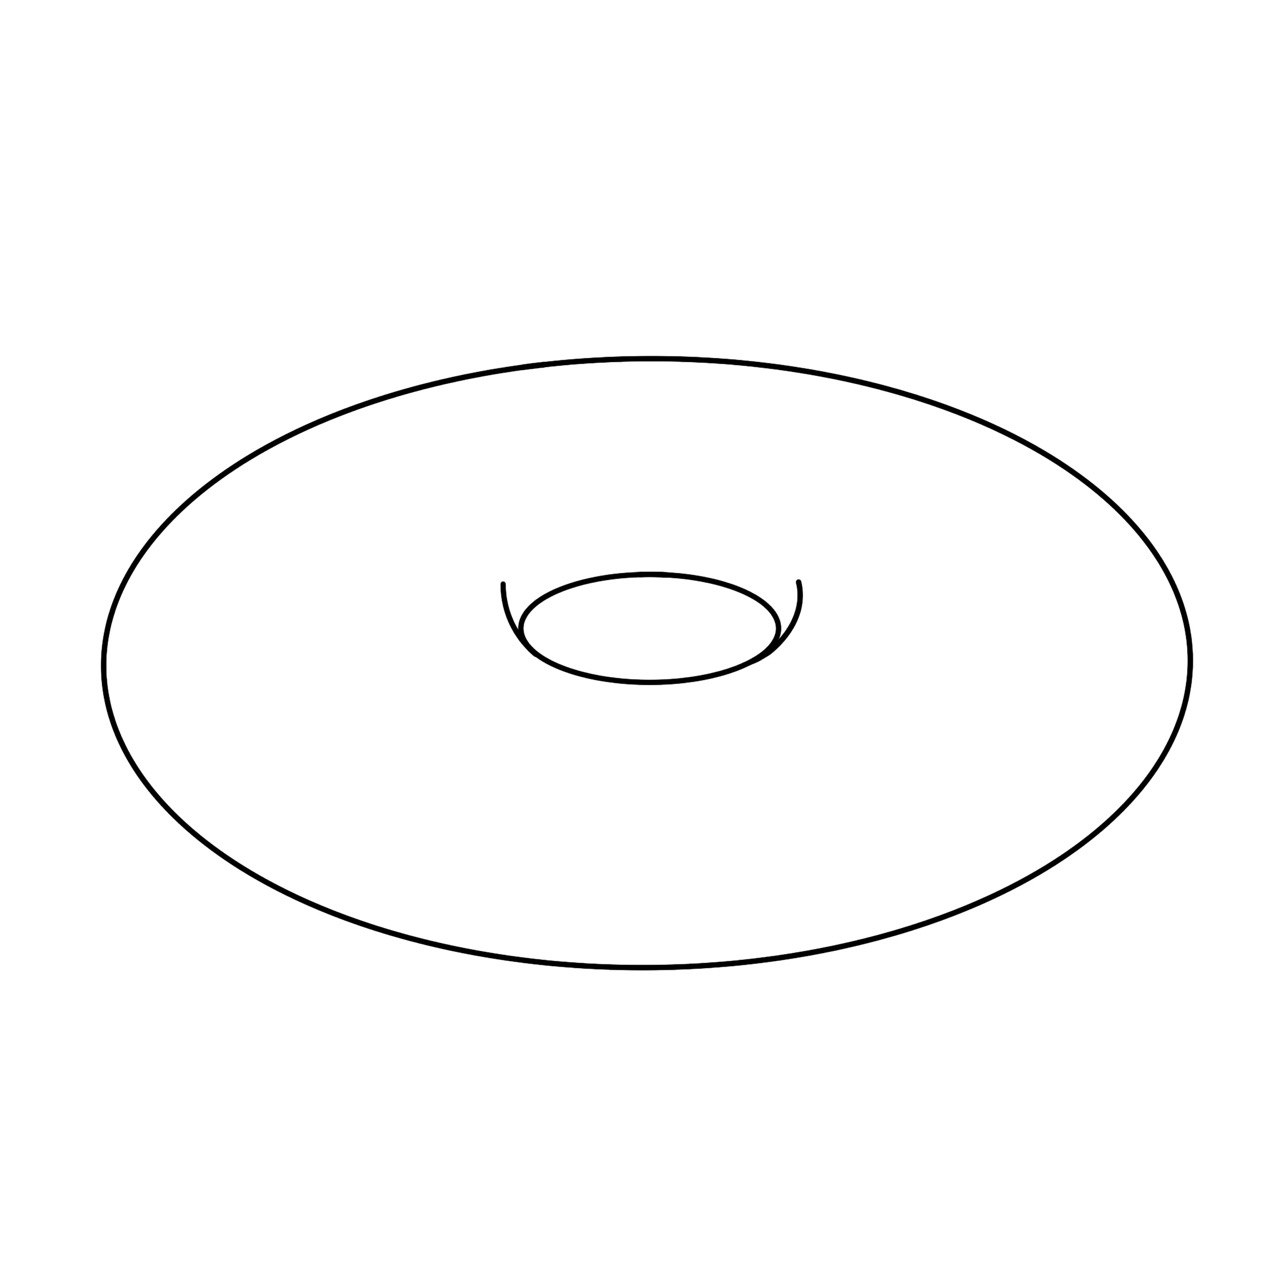
\includegraphics[width=0.5\linewidth]{images/plain torus.jpg}
    \caption{A torus}
    \label{fig:torus}
    \addtocontents{lof}{Artist: Chandler DeMarco}
\end{figure}

%Consider for a moment how the torus is essentially two perpendicular circles joined at a single point. Allow me to explain with a thought experiment.
Consider for a moment how the torus is essentially two perpendicular circles joined at a single point. This can be explored further with a thought experiment.

For a torus, there are two main types of loops: one horizontal loop around the surface of the torus, and a vertical one that passes through the hole. To better visualize these, imagine that you have two doughnuts in front of you.

%% TODO: consider rewriting this?
Now, imagine yourself deciding to frost the doughnut as precisely as you would decorate a cake. You take your pastry piping bag and carefully draw a circle of frosting around the body of the doughnut; this is the horizontal loop. Now, suppose you want to take the second doughnut and completely soak your doughnut in glaze. So, you tie a string through the hole of the doughnut so you can safely submerge it into the glaze without getting your hands all sticky. A wise move. That string you tied around it is the vertical loop we're describing.

\begin{figure}
    \centering
    \captionsetup{justification=centering}
    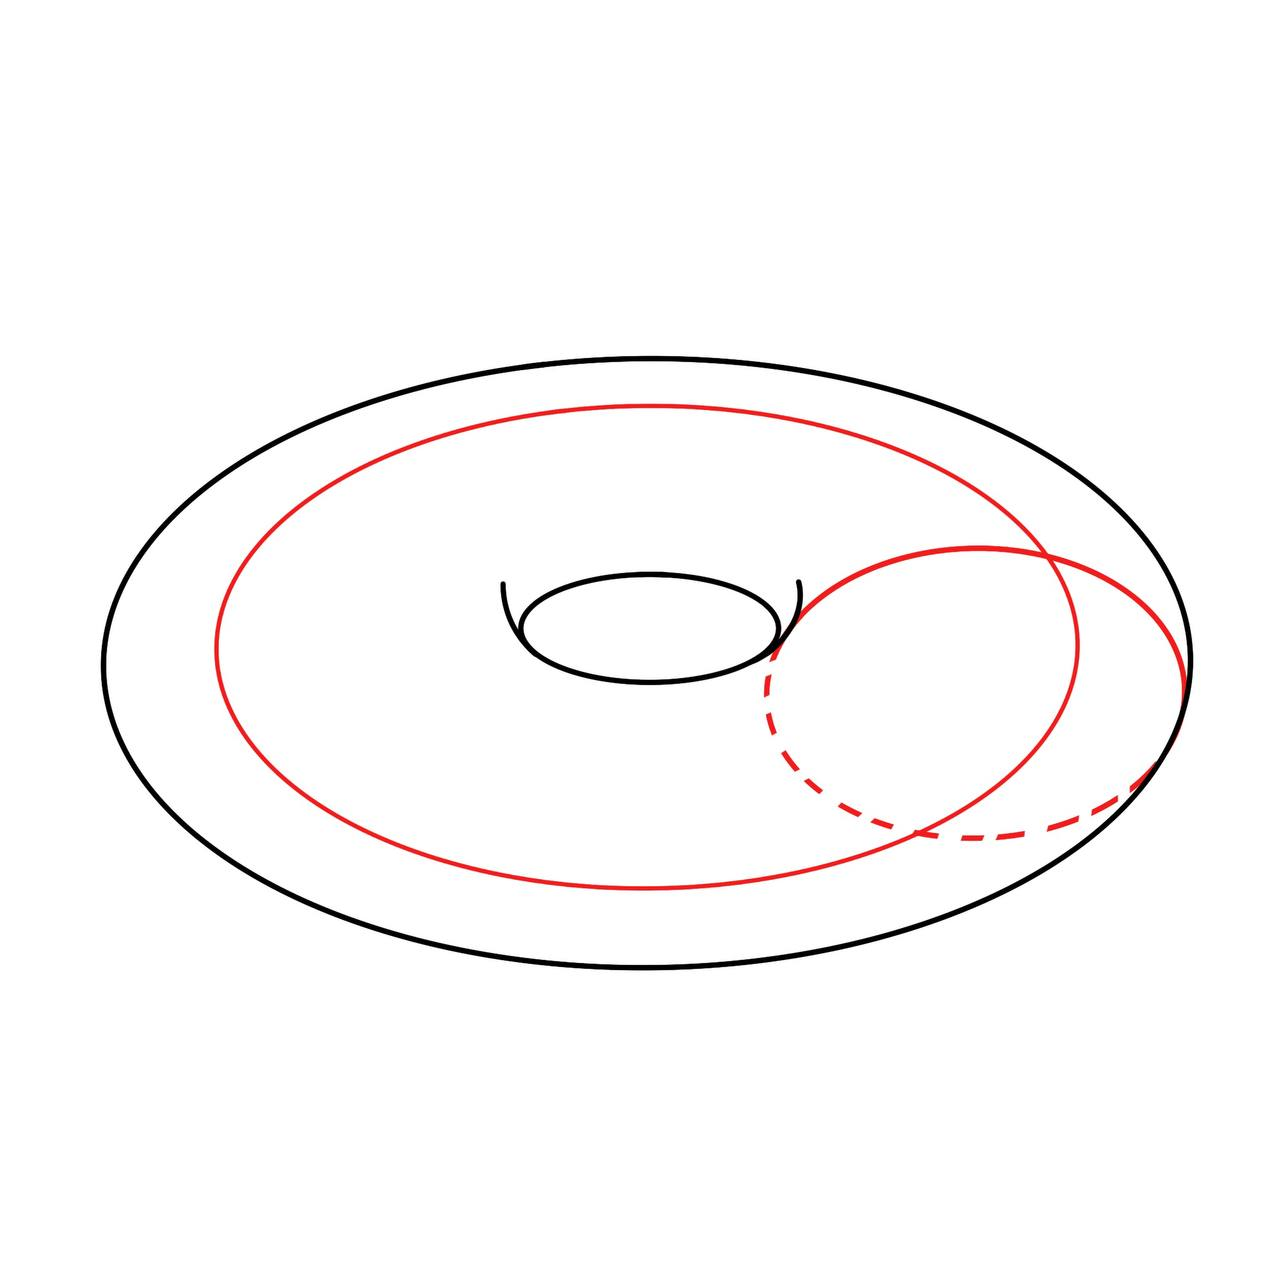
\includegraphics[width=0.5\linewidth]{images/torus with curves.jpg}
    \caption{A torus, with paths shown by two circles}
    \label{fig:two circles}
    \addtocontents{lof}{Artist: Chandler DeMarco}
\end{figure}

If you take the \textit{product} of these two loops, \textit{not} the cross product, we get a torus (demonstrated in Figure \ref{fig:two circles}). The horizontal loop and the vertical loop are both circles, so we can call both of them $S^1$. Their product becomes $S^1\times S^1$, which looks awfully similar to the cross product notation, but do not be deceived. We know $S^1=\{z\in\C\mid|z|=1\}$, and the corresponding fundamental group is $\pi_1(S^1)\simeq\Z$. Thus, we would have
\[\pi_1(S^1\times S^1)\simeq\pi_1(S^1)\times\pi_1(S^1)\simeq\Z\times\Z,\]
which gives us the fundamental group of the torus: $\pi_1(T)\simeq\Z\times\Z.$

\section{Covering a Torus}

To further analyze the torus, we consider its universal covering. To construct the universal covering of a torus, take a torus, a doughnut if you will, and cover it with wrapping paper. When unfolded and flattened out, the wrapping paper used to cover your doughnut (torus) takes on a rectangular shape.

Let's move backwards to better visualize this. Imagine a sheet of printer paper that you can stretch and pull easily. If you glue two opposite sides together, you would have a cylindrical tube. Then, imagine taking the two circular bases of this cylinder and gluing them together. Then you have a torus.\\

\centerline{\begin{tikzpicture}[]
\begin{scope}[very thick,decoration={markings,
    mark=at position 0.5 with {\arrow{>>}}}] 
    \draw[postaction={decorate}] (0,0)--(3,0) node[midway,above]{b};
    \draw[postaction={decorate}] (0,2)--(3,2);
\end{scope}
\begin{scope}[very thick,decoration={markings,
    mark=at position 0.5 with {\arrow{>}}}] 
    \draw[postaction={decorate}] (3,0)--(3,2);
    \draw[postaction={decorate}] (0,0)--(0,2) node[midway,left]{a};
\end{scope}
\end{tikzpicture}}

The image pictured above is clearly the universal covering of the torus. Keep in mind that this rectangle depicted above is actually a plane, specifically $\R^2$. When choosing a covering space, one wants as universal of a definition as possible. If the universal covering for a torus was not infinitely large, then there would be some tori that are just too big to be sufficiently wrapped. Now, let us mark and label these sides $a$ and $b$, just so we can keep track of them while we move onto our next step.

Imagine taking a doughnut and creating loops out of frosting. These same loops can also be drawn on the universal covering, which we have designed, though things look a bit different. 

In order to draw a line around the outside of the torus, similar to the equator around the earth, looking at this line from above makes it clear that it is not a segment that starts and ends, but a line that connects back to itself and loops around forever. If you were to look at the torus equator at eye level, it would appear straight, like a line, and it would appear to start and end on each side of the torus, since one cannot see through the shape. Consider for a moment that the torus equator that we have drawn remains exactly the same regardless of which perspective you are viewing it from. What this tells us is that a circle of infinite radius and a line in the complex plane can have the same representation.

% A line in the complex plane? It's more likely than you think
Say we want to represent this same torus equator line on the universal covering instead of on the torus itself. This can be done by starting at a point $x_0$, pictured below on the universal covering, and tracing horizontally until an edge is reached, as below.\\

\centerline{\begin{minipage}{1.75in}
\centerline{\begin{tikzpicture}[]
\begin{scope}[very thick,decoration={markings,
    mark=at position 0.5 with {\arrow{>>}}}] 
    \draw[postaction={decorate}] (0,0)--(3,0);% node[midway,above]{b};
    \draw[postaction={decorate}] (0,2)--(3,2);
\end{scope}
\begin{scope}[very thick,decoration={markings,
    mark=at position 0.5 with {\arrow{>}}}] 
    \draw[postaction={decorate}] (3,0)--(3,2);
    \draw[postaction={decorate}] (0,0)--(0,2);
	\node[circle,fill,inner sep=1pt,label=below:$x_0$] at (2,1){};
\end{scope}\end{tikzpicture}}
\end{minipage}
\begin{minipage}{1.75in}
\centerline{\begin{tikzpicture}[]
\begin{scope}[very thick,decoration={markings,
    mark=at position 0.5 with {\arrow{>>}}}] 
    \draw[postaction={decorate}] (0,0)--(3,0);
    \draw[postaction={decorate}] (0,2)--(3,2);
\end{scope}
\begin{scope}[very thick,decoration={markings,
    mark=at position 1 with {\arrow{>}}}] 
	\draw[postaction={decorate}] (2,1)--(1,1);
\end{scope}
\begin{scope}[very thick,decoration={markings,
    mark=at position 0.5 with {\arrow{>}}}] 
    \draw[postaction={decorate}] (3,0)--(3,2);
    \draw[postaction={decorate}] (0,0)--(0,2);
	\node[circle,fill,inner sep=1pt,label=below:$x_0$] at (2,1){};
\end{scope}
\end{tikzpicture}}
\end{minipage}
\begin{minipage}{1.75in}
\centerline{\begin{tikzpicture}[]
\begin{scope}[very thick,decoration={markings,
	mark=at position 0.5 with {\arrow{>>}}}] 
    \draw[postaction={decorate}] (0,0)--(3,0);
    \draw[postaction={decorate}] (0,2)--(3,2);
\end{scope}
\begin{scope}[very thick,decoration={
    markings,
    mark=at position 1 with {\arrow{>}}}
    ] 
	\draw[postaction={decorate}] (3,1)--(2,1);
	\draw[] (2,1)--(0,1);
\end{scope}
\begin{scope}[very thick,decoration={markings,
	mark=at position 0.5 with {\arrow{>}}}] 
    \draw[postaction={decorate}] (3,0)--(3,2);
    \draw[postaction={decorate}] (0,0)--(0,2);
	\node[circle,fill,inner sep=1pt,label=below:$x_0$] at (2,1){};
\end{scope}
\end{tikzpicture}}
\end{minipage}}

Now, remember that to create our torus from the universal covering, we glue the designated sides together. Similarly, to draw this loop, we wind up on the other side of the rectangle, because they are actually the same side of the torus! Now we have a line on the universal covering that corresponds to our equator around the torus. 

Likewise, if we wanted to draw a line that passes through the hole of the torus, we simply draw another line perpendicular to our first one, like so:\\

\centerline{\begin{minipage}{1.75in}
\centerline{\begin{tikzpicture}[]
\begin{scope}[very thick,decoration={markings,
    mark=at position 0.5 with {\arrow{>>}}}] 
    \draw[postaction={decorate}] (0,0)--(3,0);% node[midway,above]{b};
    \draw[postaction={decorate}] (0,2)--(3,2);
\end{scope}
\begin{scope}[very thick,decoration={markings,
    mark=at position 0.5 with {\arrow{>}}}] 
    \draw[postaction={decorate}] (3,0)--(3,2);
    \draw[postaction={decorate}] (0,0)--(0,2);
	\node[circle,fill,inner sep=1pt,label=left:$x_0$] at (2,1){};
\end{scope}\end{tikzpicture}}
\end{minipage}
\begin{minipage}{1.75in}
\centerline{\begin{tikzpicture}[]
\begin{scope}[very thick,decoration={markings,
    mark=at position 0.5 with {\arrow{>>}}}] 
    \draw[postaction={decorate}] (0,0)--(3,0);
    \draw[postaction={decorate}] (0,2)--(3,2);
\end{scope}
\begin{scope}[very thick,decoration={markings,
	mark=at position 1 with {\arrow{>}}}] 
	\draw[postaction={decorate}] (2,1)--(2,2);
\end{scope}
\begin{scope}[very thick,decoration={markings,
    mark=at position 0.5 with {\arrow{>}}}] 
    \draw[postaction={decorate}] (3,0)--(3,2);
    \draw[postaction={decorate}] (0,0)--(0,2);
	\node[circle,fill,inner sep=1pt,label=left:$x_0$] at (2,1){};
\end{scope}
\end{tikzpicture}}
\end{minipage}
\begin{minipage}{1.75in}
\centerline{\begin{tikzpicture}[]
\begin{scope}[very thick,decoration={markings,
	mark=at position 0.5 with {\arrow{>>}}}] 
    \draw[postaction={decorate}] (0,0)--(3,0);
    \draw[postaction={decorate}] (0,2)--(3,2);
\end{scope}
\begin{scope}[very thick,decoration={markings,
    mark=at position 1 with {\arrow{>}}}] 
	\draw[postaction={decorate}] (2,0)--(2,1);
	\draw[] (2,1)--(2,2);
\end{scope}
\begin{scope}[very thick,decoration={markings,
	mark=at position 0.5 with {\arrow{>}}}] 
    \draw[postaction={decorate}] (3,0)--(3,2);
    \draw[postaction={decorate}] (0,0)--(0,2);
	\node[circle,fill,inner sep=1pt,label=left:$x_0$] at (2,1){};
\end{scope}
\end{tikzpicture}}
\end{minipage}}

Now, we're going to remove one point on the surface of the torus, which does not present too many significant changes to anything already discussed. Topologically, a punctured torus is hardly different from an intact torus. Upon inspection, you'll notice that the universal covering for an intact torus still sufficiently covers a punctured torus, only now that one point that we removed when we punctured the torus is obviously no longer part of the torus, but $\R^2$ still covers it anyway, since $\R^2$ as a covering was designed for a torus will \textit{all} of its points intact. 

\begin{figure}
    \centering
    \captionsetup{justification=centering}
    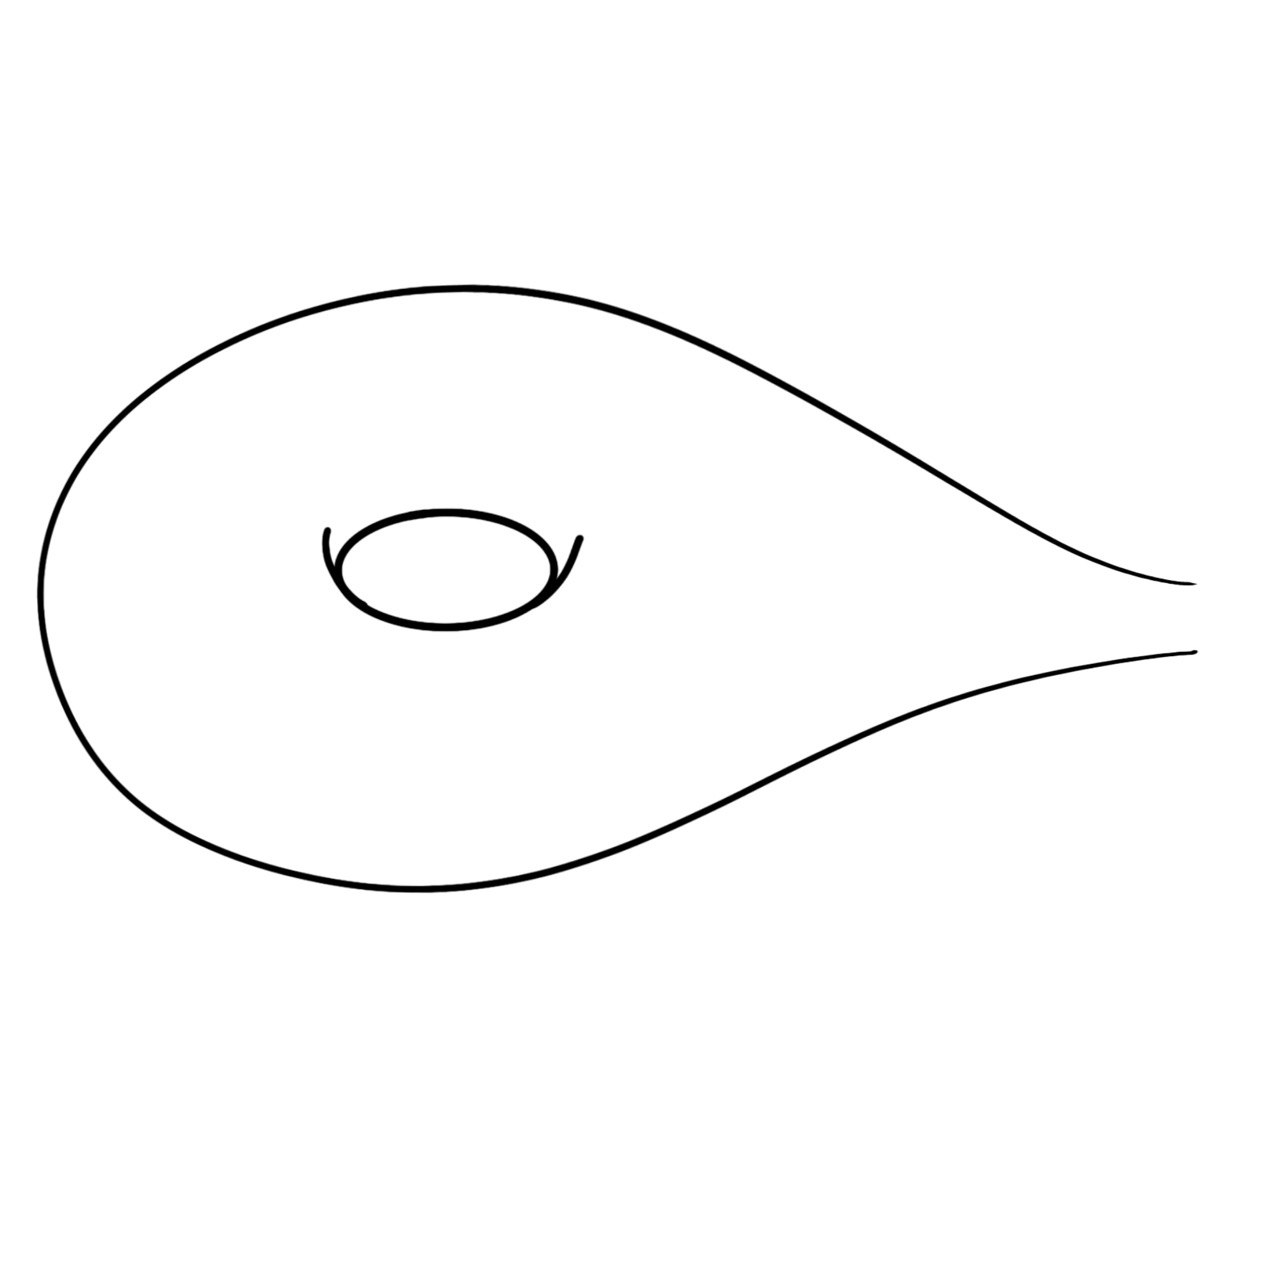
\includegraphics[width=0.5\linewidth]{images/punctured torus.jpg}
    \caption{A once-punctured torus}
    \addtocontents{lof}{Artist: Chandler DeMarco}
    \label{fig:once punctured}
\end{figure}


This can be solved by simply removing a point from the universal covering. Then our covering would look like the following:\\

\centerline{\begin{tikzpicture}[]
\begin{scope}[very thick,decoration={markings,
	mark=at position 0.525 with {\arrow{>>}}}] 
    \draw[postaction={decorate}] (0,0)--(3,0);
    \draw[postaction={decorate}] (0,2)--(3,2);
\end{scope}
\begin{scope}[very thick,decoration={markings,
    mark=at position 0.75 with {\arrow{>>>}}}] 
	\draw[postaction={decorate}] (0,0)--(3,2);
\end{scope}
\begin{scope}[very thick,decoration={markings,
    mark=at position 0.25 with {\arrow{>>>}}}] 
	\draw[-o] (0,0)--(1.5,1);
\end{scope}
\begin{scope}[very thick,decoration={markings,
	mark=at position 0.5 with {\arrow{>}}}] 
    \draw[postaction={decorate}] (3,0)--(3,2);
    \draw[postaction={decorate}] (0,0)--(0,2);
\end{scope}
\end{tikzpicture}}


Additionally, recall that the choice of basepoint for a fundamental group $\pi_1(X)$ is only arbitrary when $X$ is simply connected, meaning no holes. We must avoid the origin.

We can denote a punctured torus as $T\setminus\{0,0\}$. Our choice of point to remove is arbitrary, much like with the fundamental group, so let us choose the origin for convenience. For ease of notation, $T$ will now refer to the \textit{punctured} torus, unless otherwise specified.

\section{The Riemann Sphere}

% Contemplate the orb.

The Riemann sphere is quite odd and fairly complex, but also fascinating. Its name may be a bit misleading, because we aren't talking about a sphere in the traditional sense. Instead, the Riemann sphere $\hat\C$ refers to the union between the set of complex numbers and infinity, as defined below:
\[\hat\C=\C\cup\{\infty\}.\]
An interesting detail is that here, $\infty$ is treated as a point, as would, say, $(0,0)$. 

But how are we to get from the universal covering of a torus to the Riemann sphere? Well, consider for a moment that $\R^2$ is fairly similar to $\C$. Each point $(x,y)\in\R^2$ is determined by a horizontal shift $x$ and a vertical shift $y$. Points $z=a+bi\in\C$ are also defined by a horizontal shift $a$ and a vertical shift $b$. 

Clearly, we can define a map $f:\R^2\to\C$ as $f(x,y)=x+yi$.

We can also define the inverse map $g:\C\to\R^2$ as $g(z)=(Re(z),Im(z))$, where $Re(z)=a$ and $Im(z)=b$ are the real and imaginary components of $z=a+bi$, respectively. This inverse map will be useful later, because its existence means that not only can we map the universal covering of a punctured torus to the Riemann sphere; it means we can go back, from the Riemann sphere to the universal covering of the punctured torus.

In Figure \ref{fig:universal-covering}, we have the universal covering and a projection of the tessellated covering onto the Riemann sphere, creating an infinite tiling. For our purposes, it is more effective to redraw the same image using the same initial points that were used in most of the code (Figure \ref{fig:universal-covering-2}). 

\begin{figure}
     \centering
     \captionsetup{justification=centering}
     
     \begin{subfigure}[b]{0.49\textwidth}
         \centering
         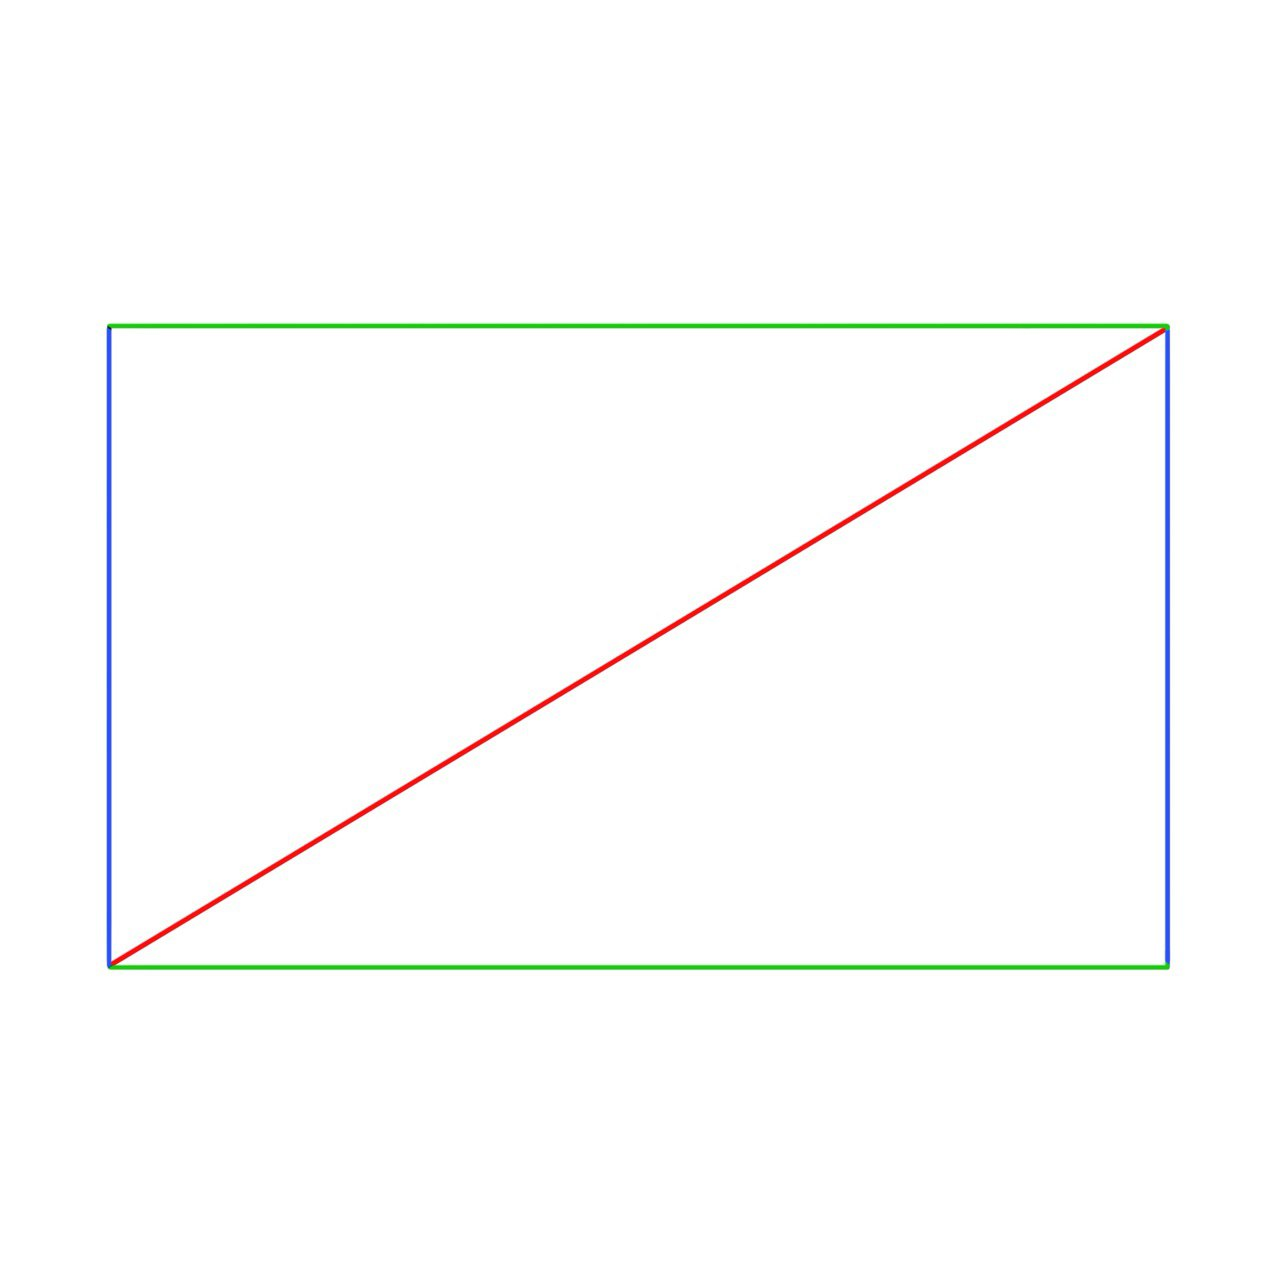
\includegraphics[width=\textwidth]{images/Universal Covering.jpg}
         \caption{Universal covering of a torus}
         \label{fig:covering}
     \end{subfigure}
     \hfill
     \begin{subfigure}[b]{0.49\textwidth}
         \centering
         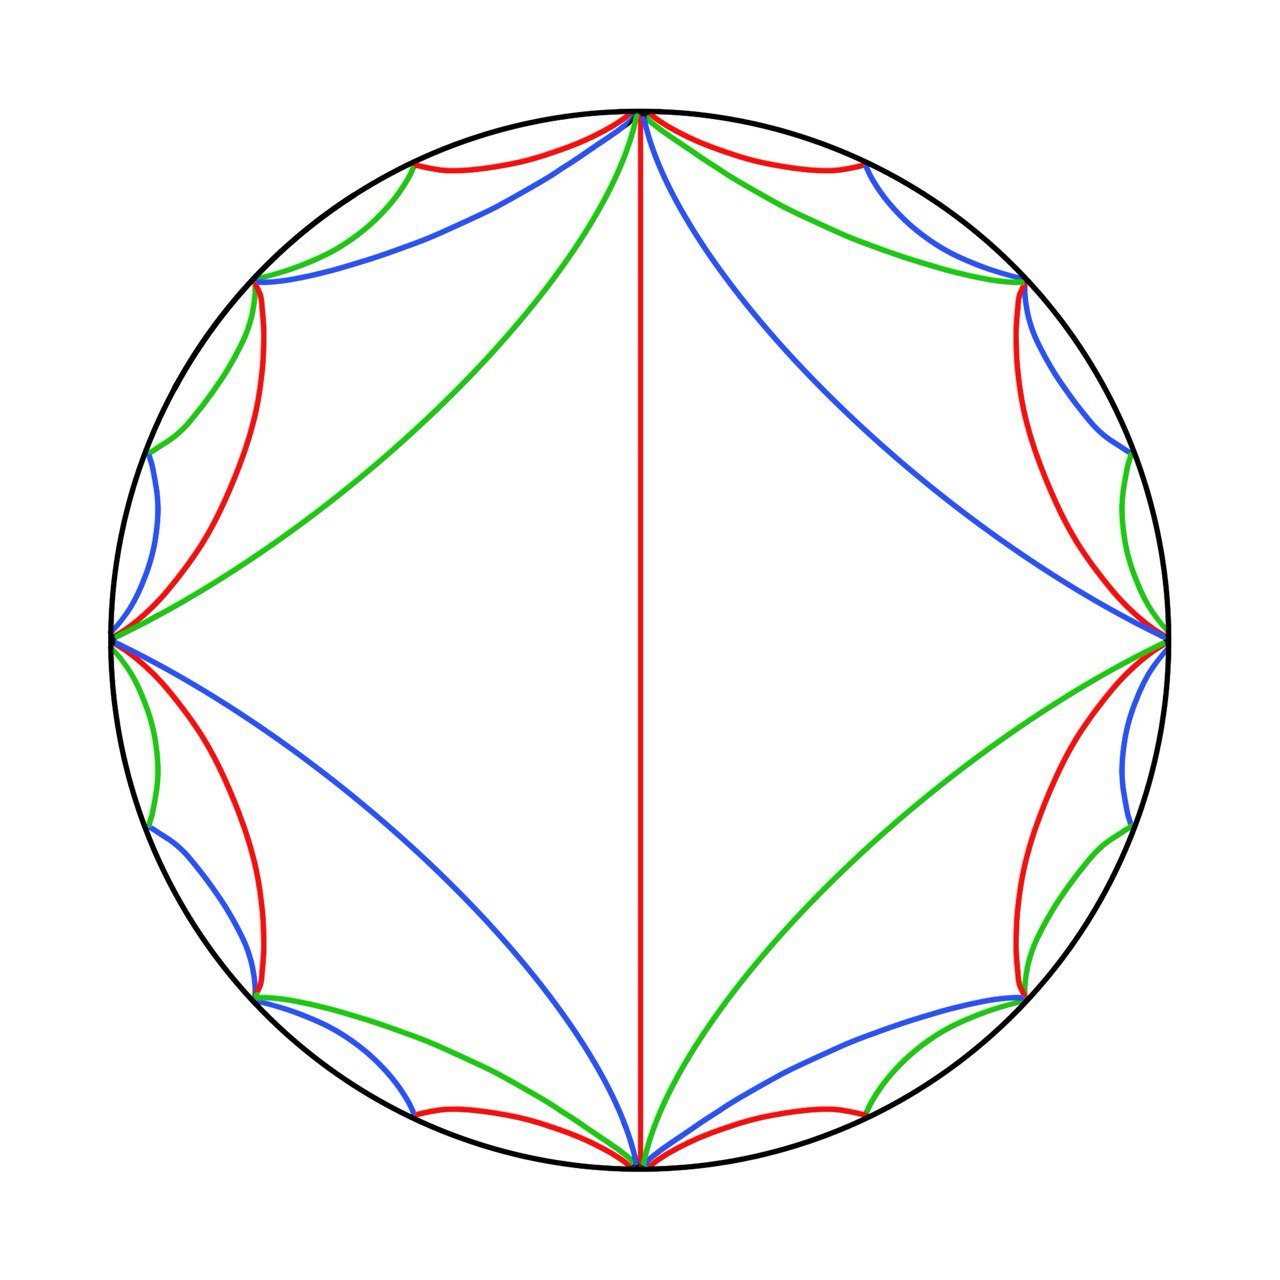
\includegraphics[width=\textwidth]{images/RS colored detailed.jpg}
         \caption{Universal covering of a torus projected onto the Riemann sphere}
         \label{fig:tesselated}
     \end{subfigure}
        \caption{Universal covering of a torus and its projection onto the Riemann sphere}
        \addtocontents{lof}{Artist: Chandler DeMarco}
        \label{fig:universal-covering}
\end{figure}


\begin{figure}
    \centering
    \captionsetup{justification=centering}
    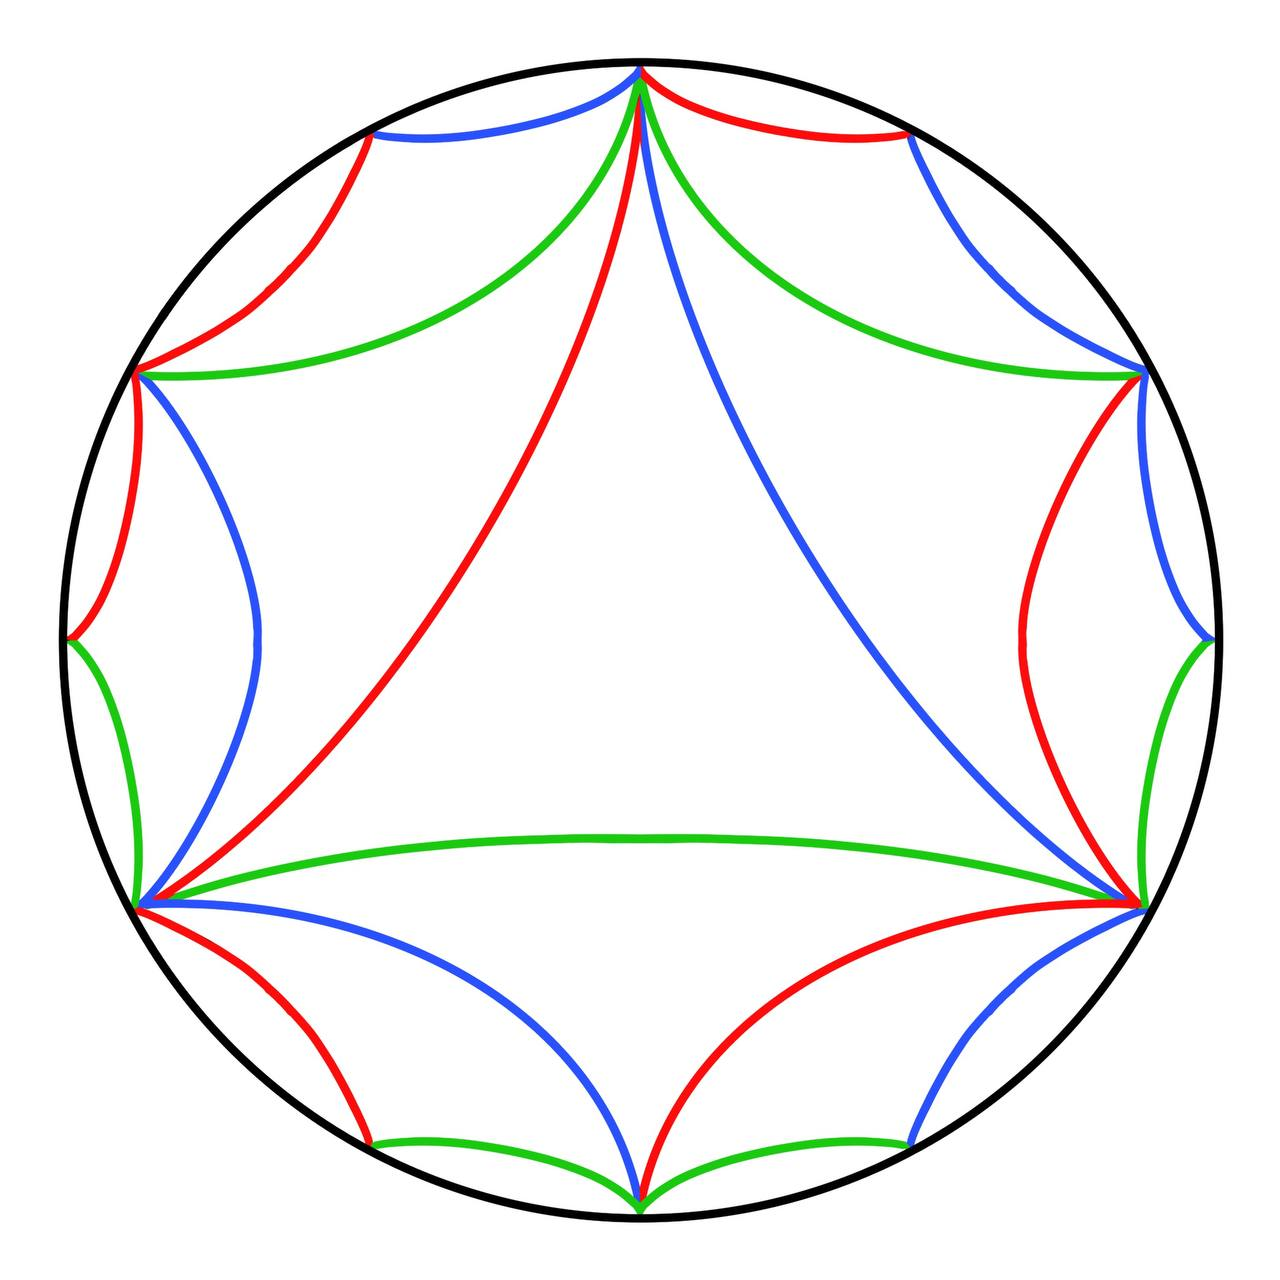
\includegraphics[width=0.5\textwidth]{images/RS colored detailed 2.jpg}
    \caption{Universal covering of a torus projected onto the Riemann sphere, using same initial conditions as this project}
    \addtocontents{lof}{Artist: Chandler DeMarco}
    \label{fig:universal-covering-2}
\end{figure}

\section{Möbius Transformations}

Möbius Transformations are a type of deck transformation of the form \[f(z)=\frac{az+b}{cz+d};\quad\quad ad-bc=1,\]
where $a,b,c,d$ are complex numbers. It should be noted that Möbius transforms are transitive, which means we can combine two or more Möbius transforms together to compose a larger one, just like how we can add together multiple paths to create a longer, more intricate path. Möbius transforms are also bijective, which allows them to be ``undone'' with an inverse.

A crucial property with Möbius transforms is that if you take four distinct, nonzero points on a circle, or line, since circles and lines are one in the same here on $\hat\C$, you can transform them into any other combination of four distinct, nonzero points using Möbius transforms. Below is a theorem, courtesy of a handout written by Rich Schwartz \cite{Schwartz_2007}:
\begin{theorem}Let $(z_1,z_2,z_3)$ and $(z_1^\prime,z_2^\prime,z_3^\prime)$ be triplets of distinct points. Then there is a unique Möbius transformation $T$ such that $T(z_1,z_2,z_3)=(z_1^\prime,z_2^\prime,z_3^\prime)$.
\end{theorem}

The above theorem looks deceptively convenient, and yet it is true. Let us consider four distinct points in $\hat\C$, $[z_1,z_2,z_3,z_4]$ and map them to $[0,1,-1,\infty]$ using a Möbius transform. Our first step will be to convert everything into convenient matrices:
\begin{align*}
[z_1,z_2,z_3,z_4]=\left[\frac{z_1}{1},\frac{z_2}{1},\frac{z_3}{1},\frac{z_4}{1}\right]
&\implies
\begin{bmatrix}z_1 & z_2 & z_3 & z_4 \\ 1 & 1 & 1 & 1\end{bmatrix}\\
[0,1,-1,\infty]=\left[\frac{0}{1},\frac{1}{1},\frac{-1}{1},\frac{1}{0}\right]
&\implies
\begin{bmatrix}0 & 1 & -1 & 1\\ 1 & 1 & 1 & 0\end{bmatrix}
\end{align*}
Now all we need to find is a matrix $M=\begin{bmatrix}a&b\\c&d\end{bmatrix}$ such that
\begin{align*}
\begin{bmatrix}0 & 1 & -1 & 1\\ 1 & 1 & 1 & 0\end{bmatrix}=
\begin{bmatrix}a&b\\c&d\end{bmatrix}
\begin{bmatrix}z_1 & z_2 & z_3 & z_4 \\ 1 & 1 & 1 & 1\end{bmatrix}
\end{align*}

Once we have our Möbius transform matrix, we can easily map any distinct four points to $[0,1,-1,\infty]$. Now, what if we wanted to map $[z_1,z_2,z_3,z_4]$ to $[w_1,w_2,w_3,w_4]$?

All we need to do next is find the $M_z$ matrix maps our points $[z_1,z_2,z_3,z_4]$ to $[0,1,-1,\infty]$ and likewise find the $M_w$ that maps $[w_1,w_2,w_3,w_4]$ to $[0,1,-1,\infty]$. Then we take the inverse of $M_w$, which is simply $M_w^{-1}=\left[\begin{smallmatrix}d&-b\\-c&a\end{smallmatrix}\right]$, and combine these together. Thus,
\begin{align*}
[z_1,z_2,z_3,z_4]\xrightarrow{\text{\;\;$M_z$\;\;}}[0,1,-1,\infty]\xrightarrow{\text{\;\;$M_w^{-1}$\;}}[w_1,w_2,w_3,w_4].
\end{align*}
 Clearly, the Möbius transform that sends $[z_1,z_2,z_3,z_4]$ to $[w_1,w_2,w_3,w_4]$ is
\[M=M_z\circ M_w^{-1}.\]
The relationship between four distinct points is represented by a cross-ratio, which is unique to the ordering of the points. Thus, changing the order of the points changes the cross-ratio, which has been somewhat convenient during my coding process. Changing the ordering of the points in the cross-ratio calculation is how I was able to get my function to change directions.

When plotting our first three points on the circle, we have a triangle with vertices $F$, $A$, and $L$ where
{$F=(0,1)$, $A=\left(\sfrac{\sqrt3}{2},\sfrac{-\sqrt3}{2}\right)$, $L=\left(\sfrac{-\sqrt3}{2},\sfrac{-\sqrt3}{2}\right)$}. Note that choice of initial points is arbitrary, and these three points were selected simply because they form a symmetrical triangle on the circle.

Paths and loops on this modified version of the universal covering is similar to how paths and loops work on the torus universal covering, you start at a point on $B$ and regardless of which edge you cross, you enter $A$. the orientation is important. the side you enter in is the one that determines your next possible moves. Now that we're in $A$, say we continue in this straight line and proceed back into $B$ again. Now we are back in $B$ but this time we entered from this other side. This process repeats infinitely, though an iteration counter is used to limit the number of points plotted.

For testing purposes, the cross-ratio initially used was 1, hence no imaginary component and hence we would have the product of each sides' cross-ratio equal to 1. When the product of all three sides is $1$, we get points on a circle.

\section{Analysis}

I have included several images in the following section to be thorough and to provide a detailed account of how the different cross-ratios interact with each other. 

The three initial points used for the following images are 
$(0,1)$, $\left({\sqrt{3}}/{2},{-\sqrt{3}}/{2}\right)$, and $\left({-\sqrt{3}}/{2},{-\sqrt{3}}/{2}\right)$.
The unit circle is present on images to show deviation from the default curve created using three cross-ratios all equal to $1$.

The idea was to use a recursive function to plot the points. There were two conditions to stop the function from running: one is the number of iterations, and the other is the distance between the points. For the first case, the iteration variable is increased by 1 each time the function is called after its initial calling, and once it reaches the specified limit, the function ceases instead of calling itself again. In the second case, a distance is specified. When a new point is calculated, the distance between that new point and its parent points are evaluated, and if the distance between them is still greater than the limit we want, the function is called again to plot more. Otherwise, the function is not called again.

For some cross-ratios, the distance limit does not work to sufficiently end the recursion because sometimes the function diverges. The divergence is due to the unique property of the Riemann sphere having a point at infinity, and infinity happening to be one of the points that the curves pass through or approach. See Figure \ref{fig:divergent cross-ratio} for examples on what the function looks like when it diverges. 

\begin{figure}[H]
    \centering
    \captionsetup{justification=centering}
    \includegraphics[width=0.5\linewidth]{nn/a-100 b100 h40 d0.025}
    \caption{$A=1-100i$, $B=1+100i$\\Example of divergence}
    \label{fig:divergent cross-ratio}
\end{figure}

In this first example, consider $A=B=1+mi$.
Without an imaginary component as $m=0$, three cross-ratios all equal to $1$. This results in points that lie on a circle of radius $1$, pictured in Figure \ref{fig:circle}. Then when a small imaginary component is added, giving $A=1+0.2i$ and $B=1+0.2i$ (Figure \ref{fig:warped}). For $m=1$, we have a symmetrical curve pictured below that appears to be a fractal (Figure \ref{fig:fractal}).

\begin{figure}[H]
     \centering
     \captionsetup{justification=centering,font={small}}
     
     \begin{subfigure}[b]{0.3\textwidth}
         \centering
         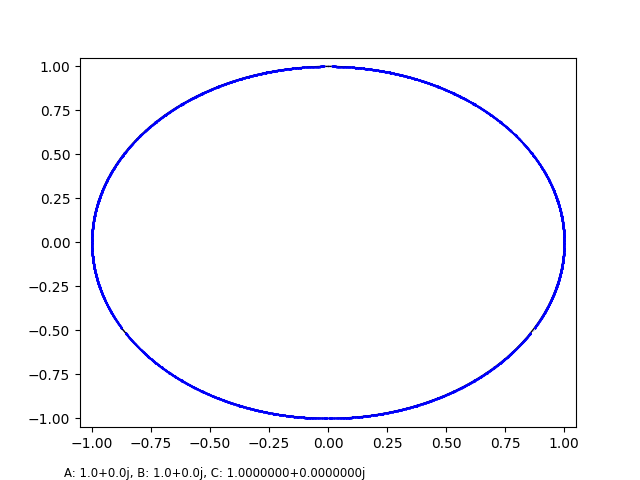
\includegraphics[width=\textwidth]{images/nn/a0 b0 h100 d0.001 auto xy.png}
         \caption{$A=1+0i$, $B=1+0i$\\Figure is a circle.}
         \label{fig:circle}
     \end{subfigure}
     \hfill
     \begin{subfigure}[b]{0.3\textwidth}
         \centering
         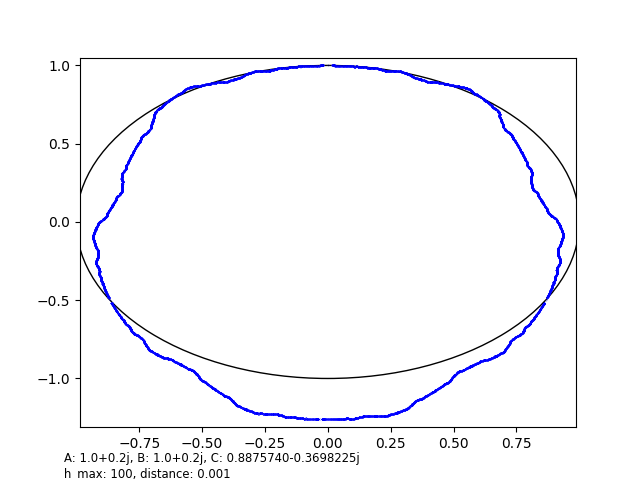
\includegraphics[width=\textwidth]{images/m/a.2,b.2,h100,d.0010.png}
         \caption{$A=1+0.2i$, $B=1+0.2i$\\Figure is slightly warped.}
         \label{fig:warped}
     \end{subfigure}
     \hfill
     \begin{subfigure}[b]{0.3\textwidth}
         \centering
         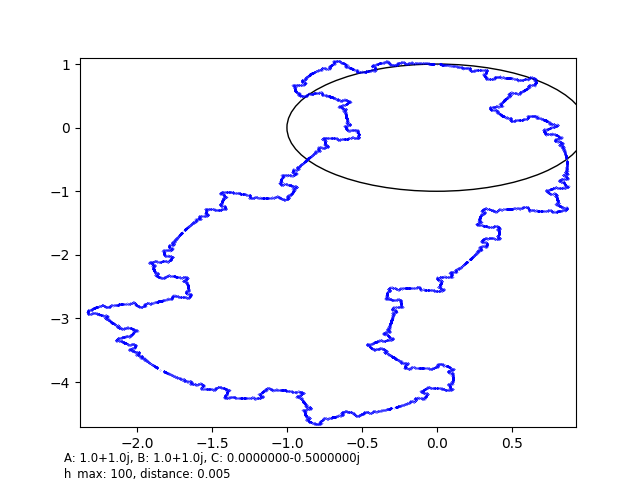
\includegraphics[width=\textwidth]{images/m/a1,b1,h100,d.005.png}
         \caption{$A=1+1i$, $B=1+1i$\\Figure resembles a fractal.}
         \label{fig:fractal}
     \end{subfigure}
     %\hfill
        \caption{Examples of small cross-ratio}
        \label{fig:small CR}
\end{figure}

Things get interesting at $m=2$. Starting with $10$ iterations, the distance between points does not mater, as only $3\cdot2^{10}=3072$ points are being plotted, which is manageable. It is only feasible to go up to $14$ iterations.  For each of the following examples, please refer to Figure \ref{fig:a2b2}, For $h=10$, that is, $10$ iterations, the faint outline of an intricate curve can be seen, though the details are lacking due to the limited number of points. For $h=11$, there is a bit more detailing as well as further divergence in the $-x$ and $-y$ direction, around $(-9,-4)$. Not much change is seen between $h=11$ and $h=12$, though more points are plotted which makes the image a bit clearer. At $h=13$, there is more divergence around $(3,3)$. At $h=14$ we see further divergence around $(-11,-4)$ and $(7,21)$. A closeup at $h=14$ has been provided to highlight the intricacies of the figure. 

\begin{figure}[H]
     \centering
     \captionsetup{justification=centering,font={small}}
     
     \begin{subfigure}[b]{0.3\textwidth}
         \centering
         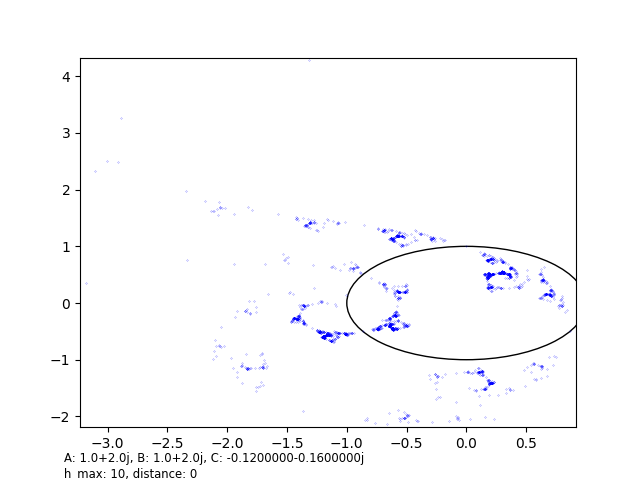
\includegraphics[width=\textwidth]{images/a2b2/a2,b2,h10,d0.png}
         \caption{$h=10$}
         \label{fig:a2b2h10}
     \end{subfigure}
     \hfill
     \begin{subfigure}[b]{0.3\textwidth}
         \centering
         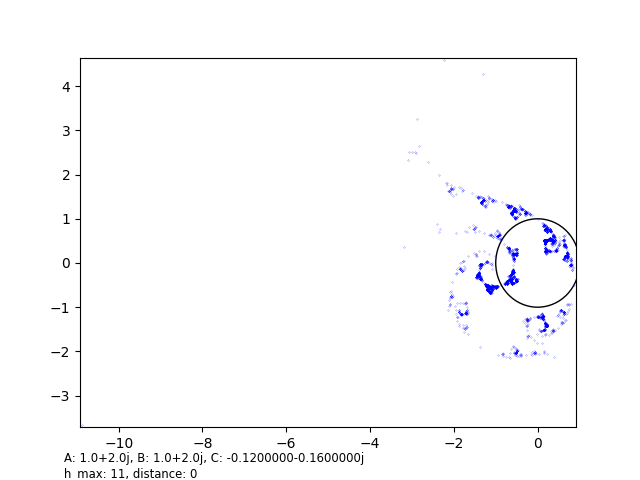
\includegraphics[width=\textwidth]{images/a2b2/a2,b2,h11,d0.png}
         \caption{$h=11$}
         \label{fig:a2b2h11}
     \end{subfigure}
     \hfill
     \begin{subfigure}[b]{0.3\textwidth}
         \centering
         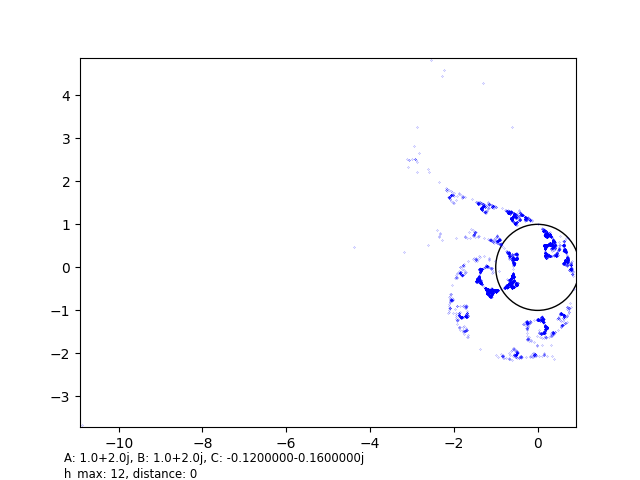
\includegraphics[width=\textwidth]{images/a2b2/a2,b2,h12,d0.png}
         \caption{$h=12$}
         \label{fig:a2b2h12}
     \end{subfigure}
     
     \begin{subfigure}[b]{0.3\textwidth}
         \centering
         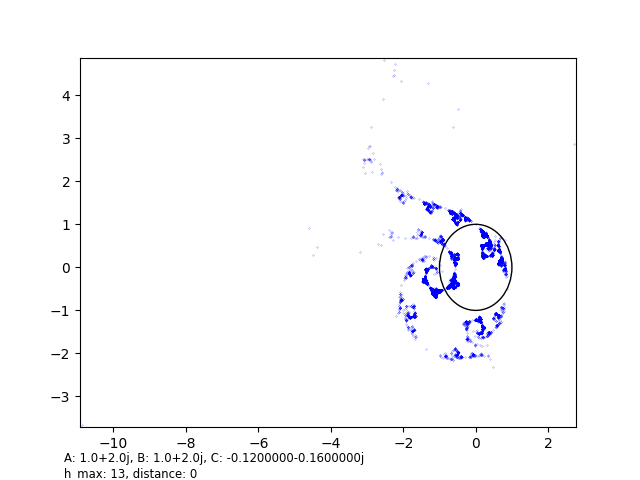
\includegraphics[width=\textwidth]{images/a2b2/a2,b2,h13,d0.png}
         \caption{$h=13$}
         \label{fig:a2b2h13}
     \end{subfigure}
     %\hfill
     \begin{subfigure}[b]{0.3\textwidth}
         \centering
         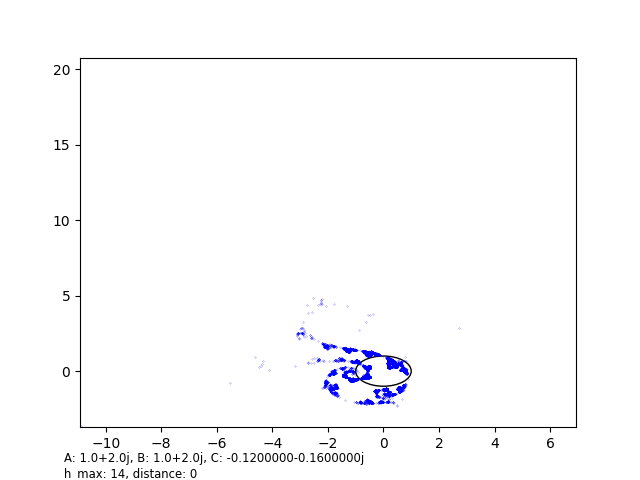
\includegraphics[width=\textwidth]{images/a2b2/a2,b2,h14,d0.png}
         \caption{$h=14$}
         \label{fig:a2b2h14}
     \end{subfigure}
     
        \caption{Examples of $A=1+2i$, $B=1+2i$}
        \label{fig:a2b2}
\end{figure}

This divergence when $m=2$ is not present for $m=3$ and instead the cross-ratios produce a fractal curve more intricate to that of $m=1$, which also connects back into itself nicely, shown in Figure \ref{fig:m}. For $m=5$, the image is similar to that of $m=3$, though it has become more jagged and angular. Continuing to $m=10$, the points are starting to tend back towards the unit circle, which becomes more obvious at $m=100$ and even more so at $m=1,000$ and $m=10,000$.

\begin{figure}[H]
     \centering
     \captionsetup{justification=centering,font={small}}
     
     \begin{subfigure}[b]{0.3\textwidth}
         \centering
         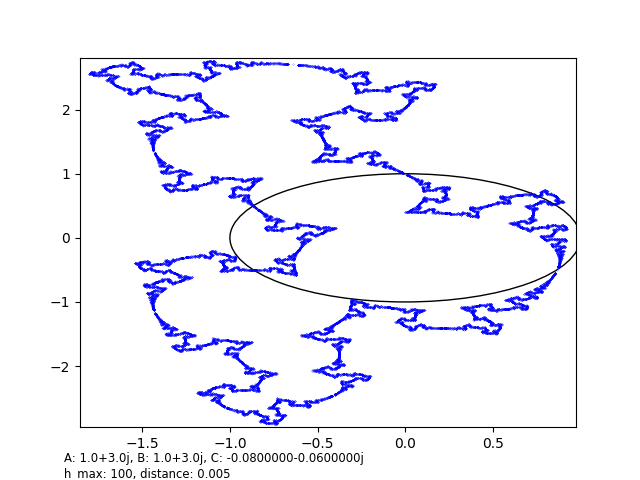
\includegraphics[width=\textwidth]{images/m/a3,b3,h100,d.005.png}
         \caption{$m=3$}
         \label{fig:m3}
     \end{subfigure}
     \hfill
     \begin{subfigure}[b]{0.3\textwidth}
         \centering
         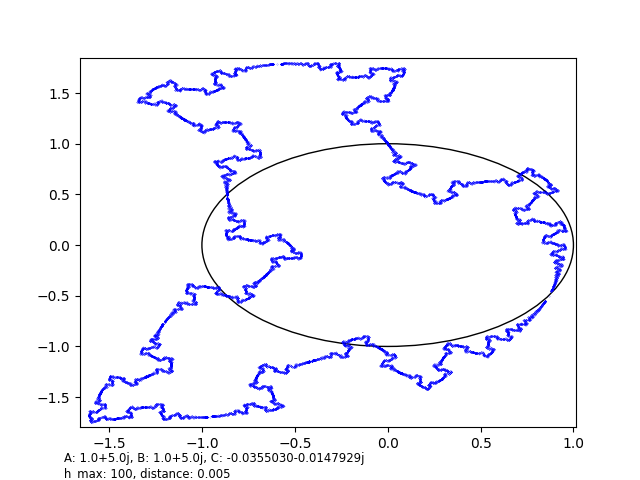
\includegraphics[width=\textwidth]{images/m/a5,b5,h100,d.005.png}
         \caption{$m=5$}
         \label{fig:m5}
     \end{subfigure}
     \hfill 
     \begin{subfigure}[b]{0.3\textwidth}
         \centering
         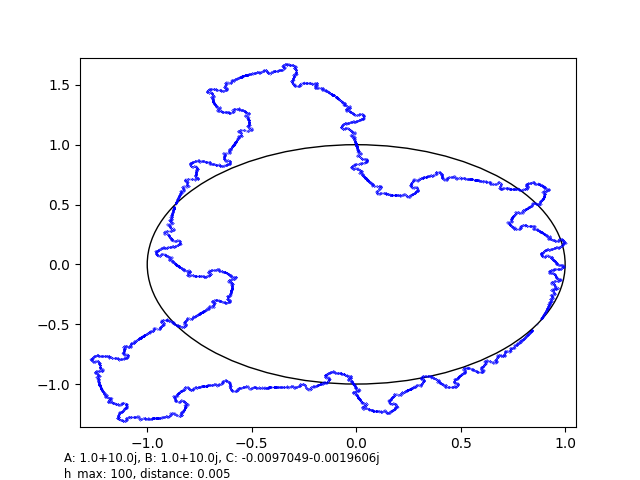
\includegraphics[width=\textwidth]{images/m/a10,b10,h100,d.005.png}
         \caption{$m=10$}
         \label{fig:m10}
     \end{subfigure}
     %\hfill
     \begin{subfigure}[b]{0.3\textwidth}
         \centering
         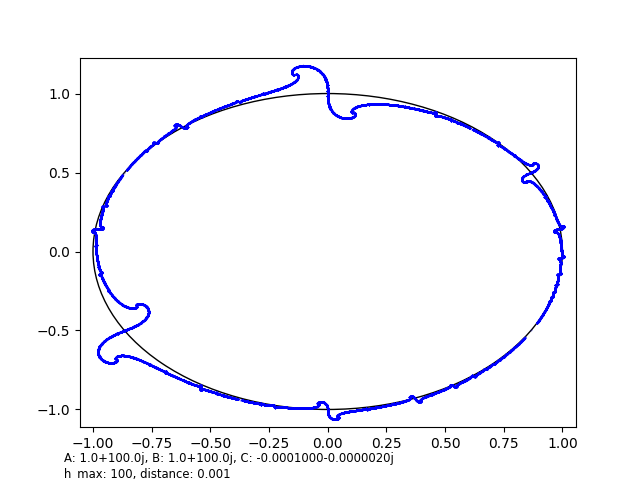
\includegraphics[width=\textwidth]{images/m/a100,b100,h100,d.0010.png}
         \caption{$m=100$}
         \label{fig:m100}
     \end{subfigure}
     \hfill
     \begin{subfigure}[b]{0.3\textwidth}
         \centering
         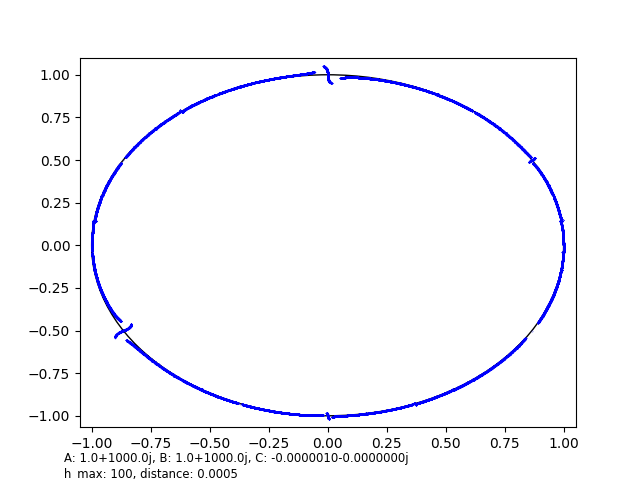
\includegraphics[width=\textwidth]{images/m/a1000,b1000,h100,d.0005.png}
         \caption{$m=1,000$}
         \label{fig:m1,000}
     \end{subfigure}
     \hfill
     \begin{subfigure}[b]{0.3\textwidth}
         \centering
         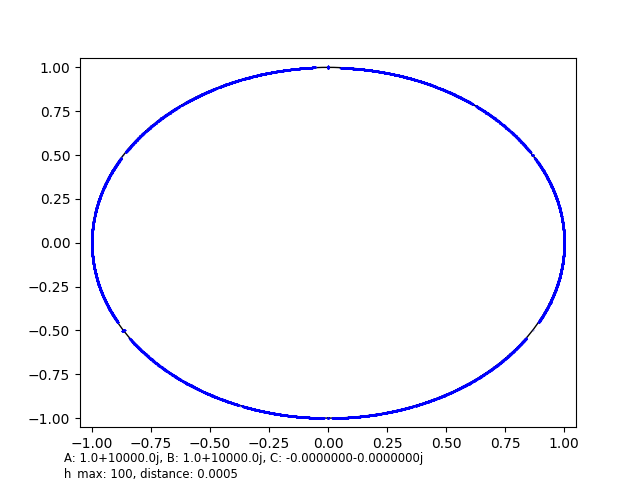
\includegraphics[width=\textwidth]{images/m/a10,000,b10,000,h100,d.0005.png}
         \caption{$m=10,000$}
         \label{fig:m10,000}
     \end{subfigure}
     
        \caption{Examples of $A=B=1+mi$, $h=100$}
        \label{fig:m}
\end{figure}

Things grow more intricate at $m=100,000$, where smaller circles are produced along the unit circle, shown below. At $m=150,000$ these circles have grown larger. By $m=1,000,000$ we see many circles that overlap and intersect with the unit circle, shown in Figures \ref{fig:large-m} and \ref{fig:large-m2}.

\begin{figure}[H]
     \centering
     \captionsetup{justification=centering,font={small}}
     
     \begin{subfigure}[b]{0.49\textwidth}
         \centering
         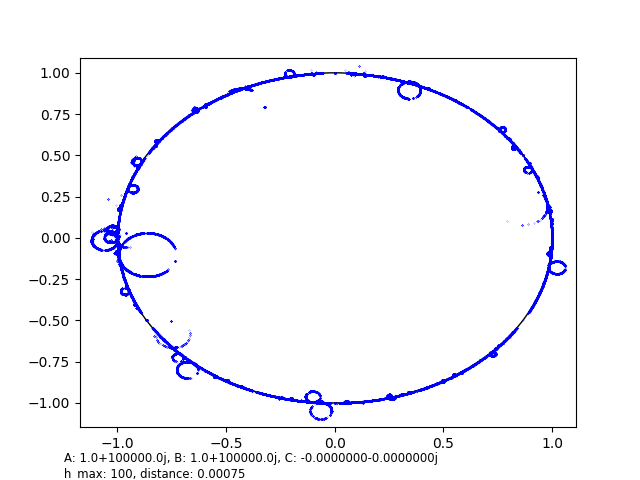
\includegraphics[width=\textwidth]{images/m/a100,000,b100,000,h100,d.00075.png}
         \caption{$m=100,000$}
         \label{fig:m100,000}
     \end{subfigure}
     \begin{subfigure}[b]{0.49\textwidth}
         \centering
         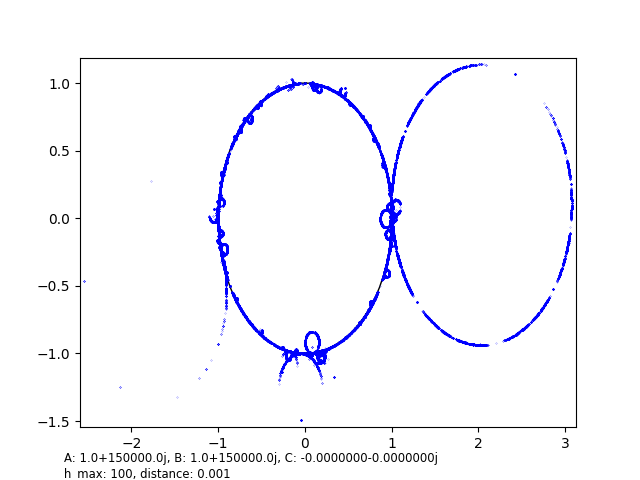
\includegraphics[width=\textwidth]{images/m/a150,000,b150,000,h100,d.0010.png}
         \caption{$m=150,000$}
         \label{fig:m150,000}
     \end{subfigure}
        \caption{Examples of $A=B=1+mi$, $h=100$, with large $m$}
        \label{fig:large-m}
\end{figure}
\begin{figure}[H]
     \begin{subfigure}[b]{0.49\textwidth}
         \centering
         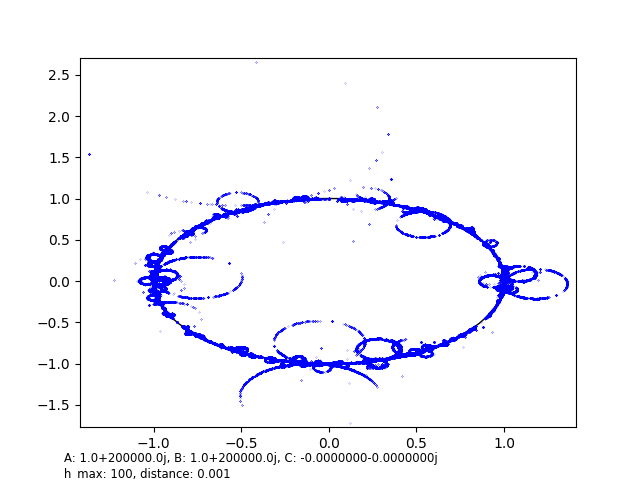
\includegraphics[width=\textwidth]{images/m/a200,000,b200,000,h100,d.0010.png}
         \caption{$m=200,000$}
         \label{fig:m200,000}
     \end{subfigure}
     \begin{subfigure}[b]{0.49\textwidth}
         \centering
         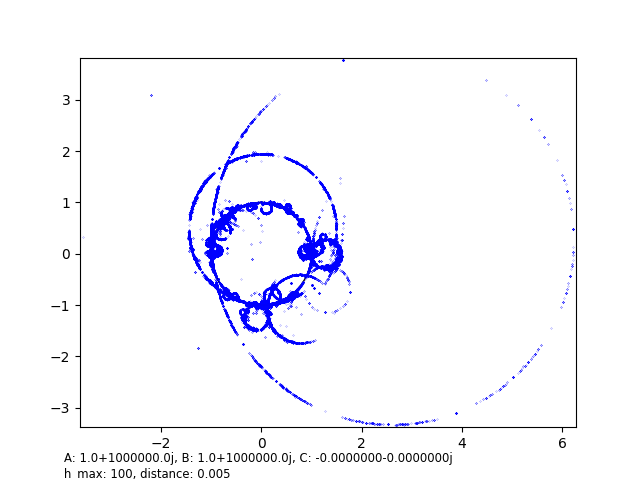
\includegraphics[width=\textwidth]{images/m/a1,000,000,b1,000,000,h100,d.005.png}
         \caption{$m=1,000,000$}
         \label{fig:m1,000,000}
     \end{subfigure}
     
        \caption{Examples of $A=B=1+mi$, $h=100$, with large $m$}
        \label{fig:large-m2}
\end{figure}

It is also important to note that the order of cross-ratios matters and leads to distinct images. Consider the below examples of $A=1+10i$, $B=1+1i$, and how that differs from $A=1+1i$, $B=1+10i$. Additionally, note that there is also divergence in $A=1+1i$, $B=1+100i$, but no such divergence in $A=1+100i$, $B=1+1i$.

\begin{figure}[H]
     \centering
     \captionsetup{justification=centering,font={small}}
     
     \begin{subfigure}[b]{.49\textwidth}
         \centering
         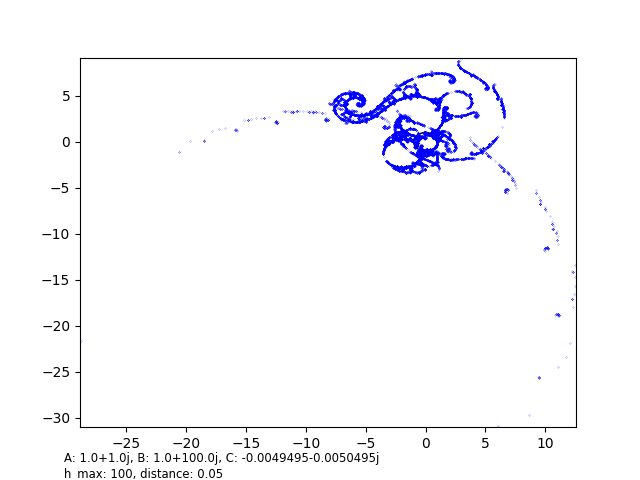
\includegraphics[width=\textwidth]{images/a1,b100,h100,d.05.png}
         \caption{$A=1+1i$, $B=1+100i$, $h=100$}
         \label{fig:a1b100}
     \end{subfigure}
     \begin{subfigure}[b]{.49\textwidth}
         \centering
        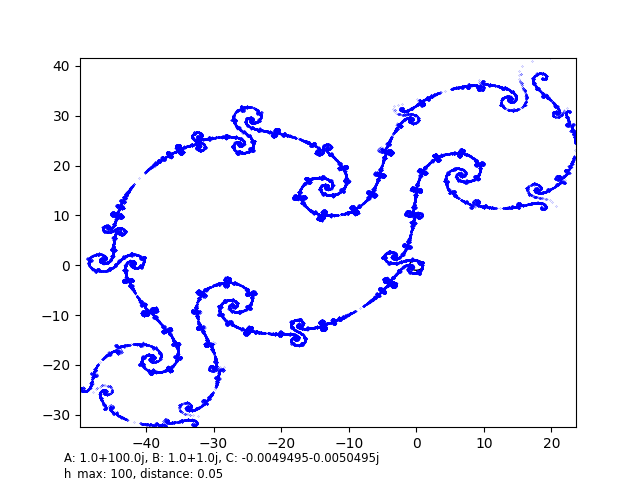
\includegraphics[width=\textwidth]{images/a100,b1,h100,d.05.png}
         \caption{$A=1+100i$, $B=1+1i$, $h=100$}
         \label{fig:a100b1}
     \end{subfigure}
        \caption{Examples of divergence with adjusted ranges}
        \label{fig:divergence-with-ranges}
\end{figure}

Some of the images appear to explode when the imaginary components of the cross-ratios get sufficiently large. This causes some issues when determining the range of the image. Since there is divergence, I have included a zoomed out version and a zoomed in version in Figure \ref{fig:divergence-with-ranges}, to present the full picture of the end behavior and also the intricacies of the details. Many of these are taken using the same bounds to show the behavior around the original three points.

\begin{figure}[H]
     \centering
     \captionsetup{justification=centering,font={small}}
     
     \begin{subfigure}[b]{\textwidth}
         \centering
         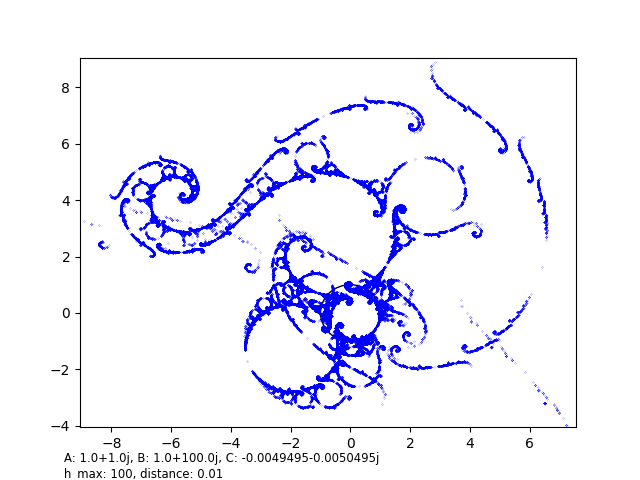
\includegraphics[width=.49\textwidth]{images/a1,b100,h100,d.01 custom xy.png}       
         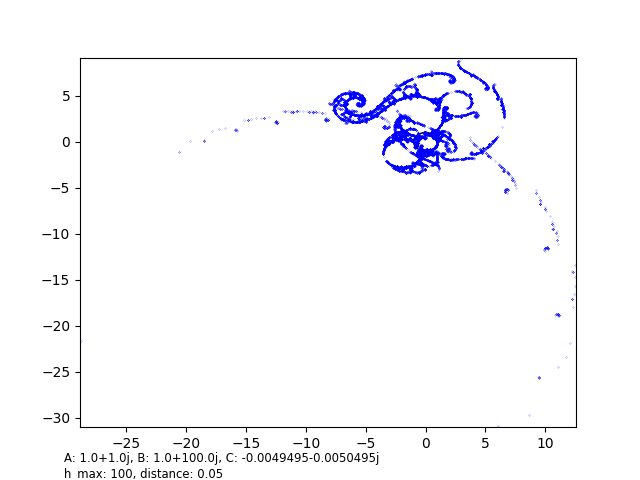
\includegraphics[width=.49\textwidth]{images/a1,b100,h100,d.05.png}
         \caption{$A=1+1i$, $B=1+100i$, $h=100$}
         \label{fig:a1b100range}
     \end{subfigure}
     \begin{subfigure}[b]{\textwidth}
         \centering
        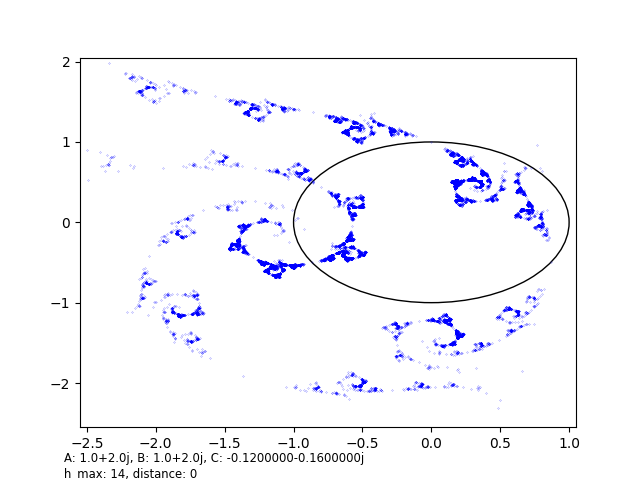
\includegraphics[width=.49\textwidth]{images/a2b2/a2,b2,h14,d0 custom bounds.png}
        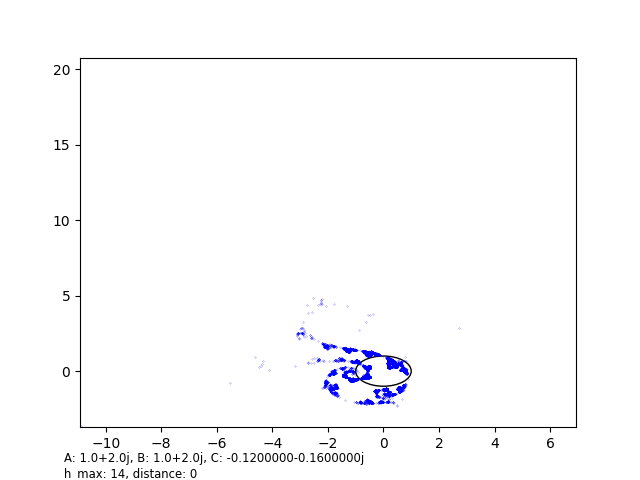
\includegraphics[width=.49\textwidth]{images/a2b2/a2,b2,h14,d0.png}
         \caption{$A=1+2i$, $B=1+2i$, $h=14$}
         \label{fig:a2b2h14range}
     \end{subfigure}
        \caption{Examples of divergence with adjusted ranges}
        \label{fig:divergence-with-ranges}
\end{figure}

Take cross-ratios $A=1-ni$ and $B=1+ni$ as an example of this. Here we have a collection of $A=1-ni$ and $B=1+ni$ with different values of $n$. In the first image, the cross-ratios are $A=1$, $B=1$, $C=1$ using $n=0$, which simply gives us a circle. From now on, I will only be referring to cross-ratios $A$ and $B$, since $C$ is not an input and is instead calculated using the relation $A\cdot B\cdot C=1$. Once the imaginary component is increased slightly to $n=1$, giving $A=1-1i$ $B=1+1i$, we find that the points no longer rest on the circle and instead form this chicken nugget-looking curve, but still a curve nonetheless. Increasing the imaginary component further, to $A=1-2i$ and $B=1+2i$ gives us another more intricate curve that still connects to itself. At $A=1-2.5i$ and $B=1+2.5i$ we see that the curve is already starting to spread out and no longer connects to itself like it did before. Increasing to $n=3$ gives $A=1-3i$ and $B=1+3i$ and causes the curve to twist and create a very interesting image. From $n=3$ to $n=5$ we see clusters of points surrounding two of the initial points, $(1,0)$ and $(-\sqrt3/2,-\sqrt3/2)$, which get tighter as $n$ increases. Near the third initial point $(\sqrt3/2,-\sqrt3/2)$, there is a gap where points avoid, which is most dramatic at $n=10$. At $n=100$ we see multiple curves that resemble waves emitting from $(\sqrt3/2,-\sqrt3/2)$.

\begin{figure}[H]
     \centering
     \captionsetup{justification=centering,font=small}
     
     \begin{subfigure}[b]{0.3\textwidth}
         \centering
         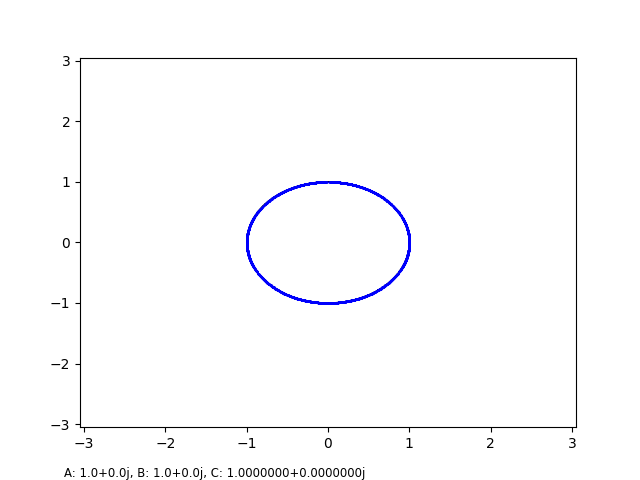
\includegraphics[width=\textwidth]{images/nn/a0 b0 h100 d0.001 fixed xy.png}
         \caption{$n=0$}
         \label{fig:n0}
     \end{subfigure}
     \hfill
     \begin{subfigure}[b]{0.3\textwidth}
         \centering
         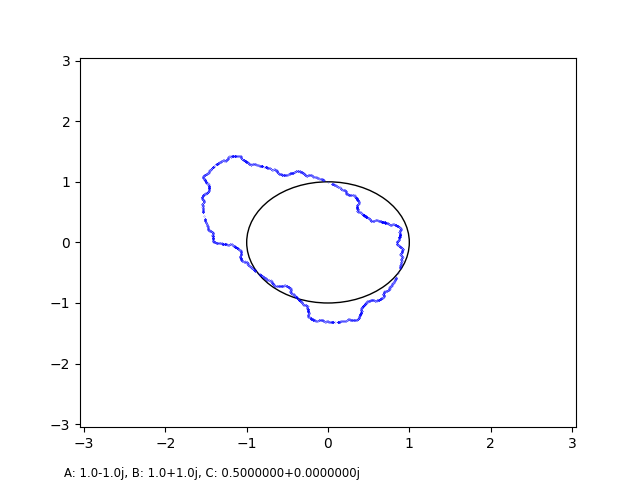
\includegraphics[width=\textwidth]{images/nn/a-1 b1 h30 d0.01.png}
         \caption{$n=1$}
         \label{fig:n1}
     \end{subfigure}
     \hfill 
     \begin{subfigure}[b]{0.3\textwidth}
         \centering
         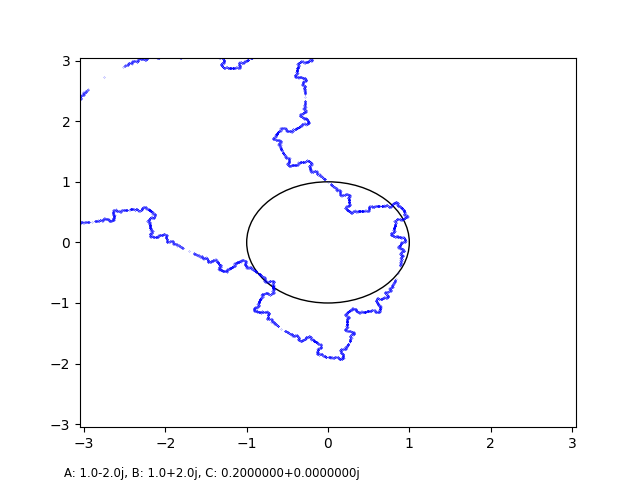
\includegraphics[width=\textwidth]{images/nn/a-2 b2 h30 d0.01.png}
         \caption{$n=2$}
         \label{fig:n2}
     \end{subfigure}
     \begin{subfigure}[b]{0.3\textwidth}
         \centering
         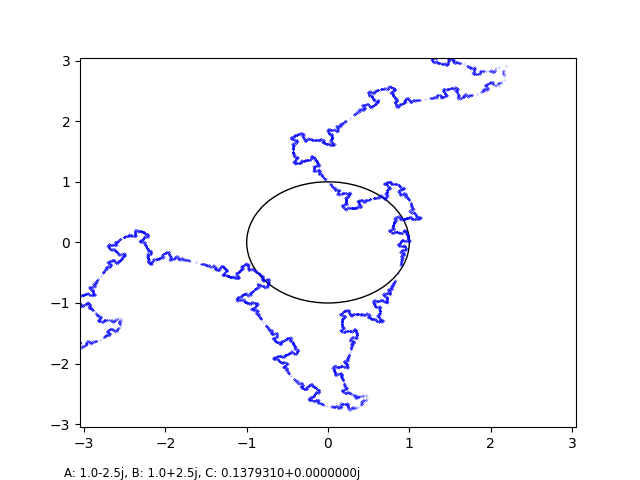
\includegraphics[width=\textwidth]{images/nn/a-2.5 b2.5 h30 d0.01.png}
         \caption{$n=2.5$}
         \label{fig:n2.5}
     \end{subfigure}
     \hfill
     \begin{subfigure}[b]{0.3\textwidth}
         \centering
         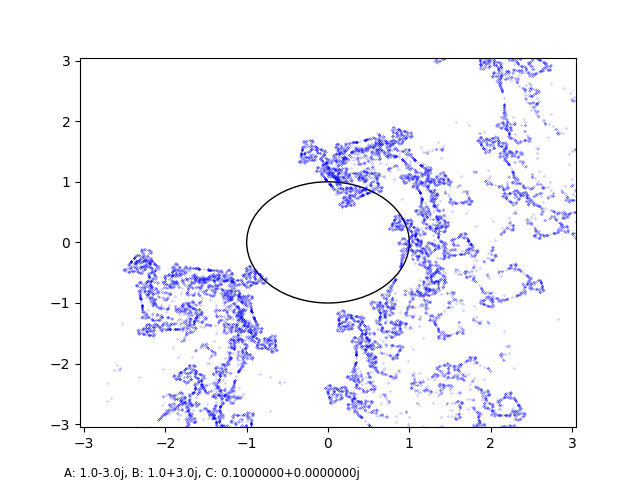
\includegraphics[width=\textwidth]{images/nn/a-3 b3 h40 d0.025.png}
         \caption{$n=3$}
         \label{fig:n3}
     \end{subfigure}
     \hfill 
     \begin{subfigure}[b]{0.3\textwidth}
         \centering
         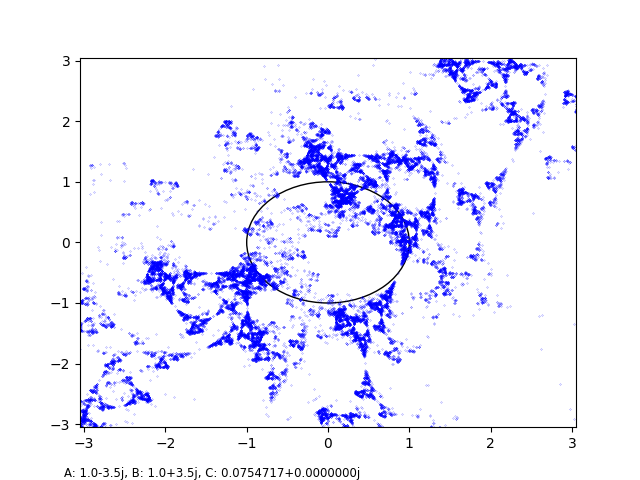
\includegraphics[width=\textwidth]{images/nn/a-3.5 b3.5 h30 d0.01.png}
         \caption{$n=3.5$}
         \label{fig:n3.5}
    \end{subfigure}
     \begin{subfigure}[b]{0.3\textwidth}
         \centering
         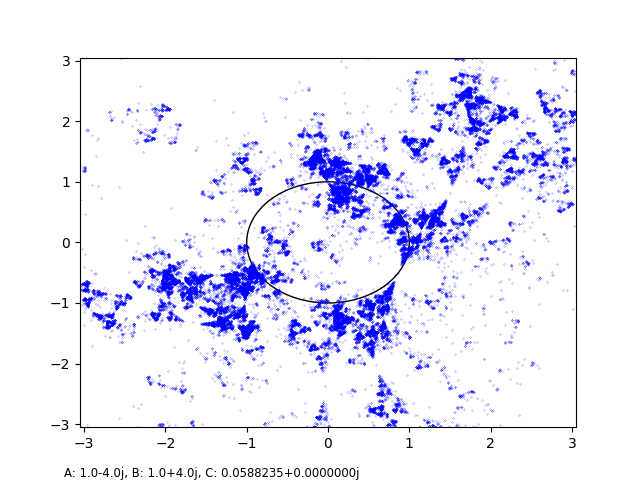
\includegraphics[width=\textwidth]{images/nn/a-4 b4 h30 d0.01.png}
         \caption{$n=4$}
         \label{fig:n4}
     \end{subfigure}
     \hfill
     \begin{subfigure}[b]{0.3\textwidth}
         \centering
         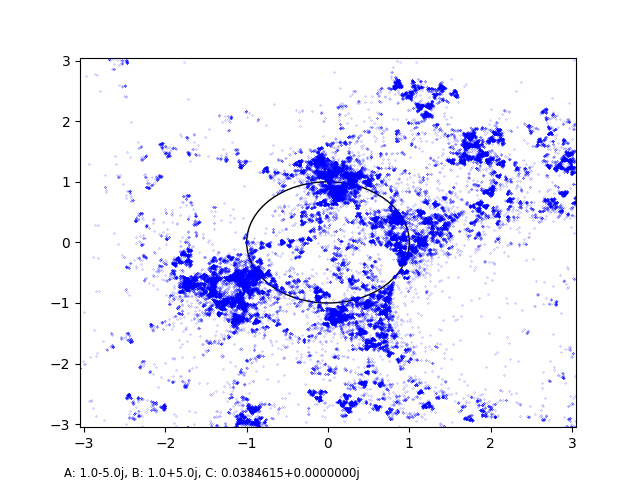
\includegraphics[width=\textwidth]{images/nn/a-5 b5 h30 d0.01.png}
         \caption{$n=5$}
         \label{fig:n5}
     \end{subfigure}
     \hfill 
     \begin{subfigure}[b]{0.3\textwidth}
         \centering
         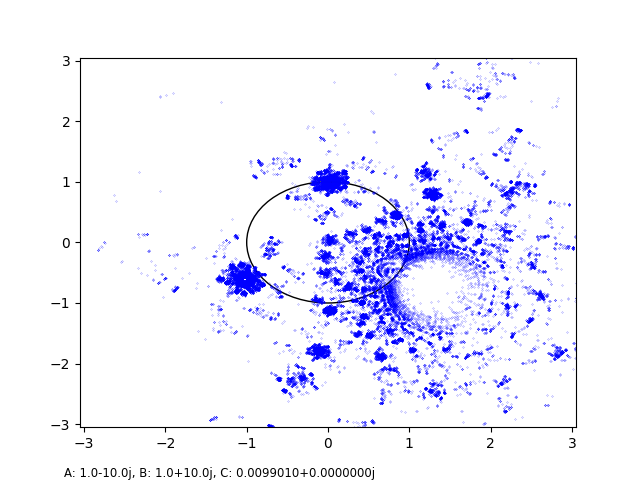
\includegraphics[width=\textwidth]{images/nn/a-10 b10 h30 d0.01.png}
         \caption{$n=10$}
         \label{fig:n10}
    \end{subfigure}
     \begin{subfigure}[b]{0.3\textwidth}
         \centering
         \includegraphics[width=\textwidth]{images/nn/a-100 b100 h40 d0.025.png}
         \caption{$n=100$}
         \label{fig:n100}
    \end{subfigure}
    \caption{Examples of $A=B=1+mi$, $h=100$, with large $m$}
    \label{fig:nn}
\end{figure}


\section{Future Work}

There are a few areas which could have been explored further given additional time and compute resources. For example, if different initial points were chosen or the product of the cross-ratio coordinates wasn't one, the patterns generated would have been completely different. Even just exploring more combinations of cross-ratios or more negative cross-ratios would have potentially revealed additional patterns in the data. The last area with room for improvement is the code itself which was used to generate the images. There were times (around 15 iterations) when the calculation time hit over 30 minutes, which severely restricted the ability to run arbitrary cross-ratios for high iteration counts. Instead, each cross-ratio set would have to be checked at a lower iteration count to ensure the resulting figure converged. Access to more compute power (for convergent, but complex scenarios) or better divergence detection (for earlier backoff) would allow future work to be explored with fewer limits.

\section{Conclusion}

In this paper, the limit sets of over 30 cross-ratio coordinate sets were computed (within the limits of the hardware used). This information allows one to extrapolate what might happen given a set of cross-ratio coordinates working from the Riemann sphere, for the set initial conditions. Although several of these patterns revealed convergent curves of varying complexity, there is a tendency for some cross-ratio coordinates to diverge. This is due to the presence of infinity on the Riemann sphere, but warrants further exploration on its own given the variety of values we see this occur with (ex. $A=1+2i$, $B=1+2i$, but also $A=1+1i$, $B=1+100i$). 

%choose different initial points
%scenario where the product of cross-ratio coordinates wasn't one
%find a way to determine more points in a divergent scenario
%optimize the code so it can exceed current limits (around 100k points or 14 iterations)
%explore more combinations of cross-ratios
%explore more with negative cross-ratios


\newpage
\appendix
\appendixpage
\addappheadtotoc

\section{Code}
Please find below the code written to plot the points (an up-to-date version is kept \href{https://github.com/scerbone121/ma499report/blob/main/circles3.py}{here}, on GitHub.

Note that it is unwise to plot more than $14$ iterations without specifying a distance value, since the program plots $3\cdot2^n$ points for $n$ iterations. Also note that due to the potential for divergence, sometimes even specifying a distance is not enough to limit the number of points. It is most efficient to plot $10$ iterations at a distance of $0$ and gradually increase the iterations from there to check for divergence first before specifying a distance and increasing the iteration count. 

\lstinputlisting[language=Python]{circles3.py}

\newpage
\bibliography{refs}

\newpage
\listoffigures

\newpage
\section{Full Images}

This section contains the full-sized images from previous figures.

\begin{figure}[H]
    \centering
    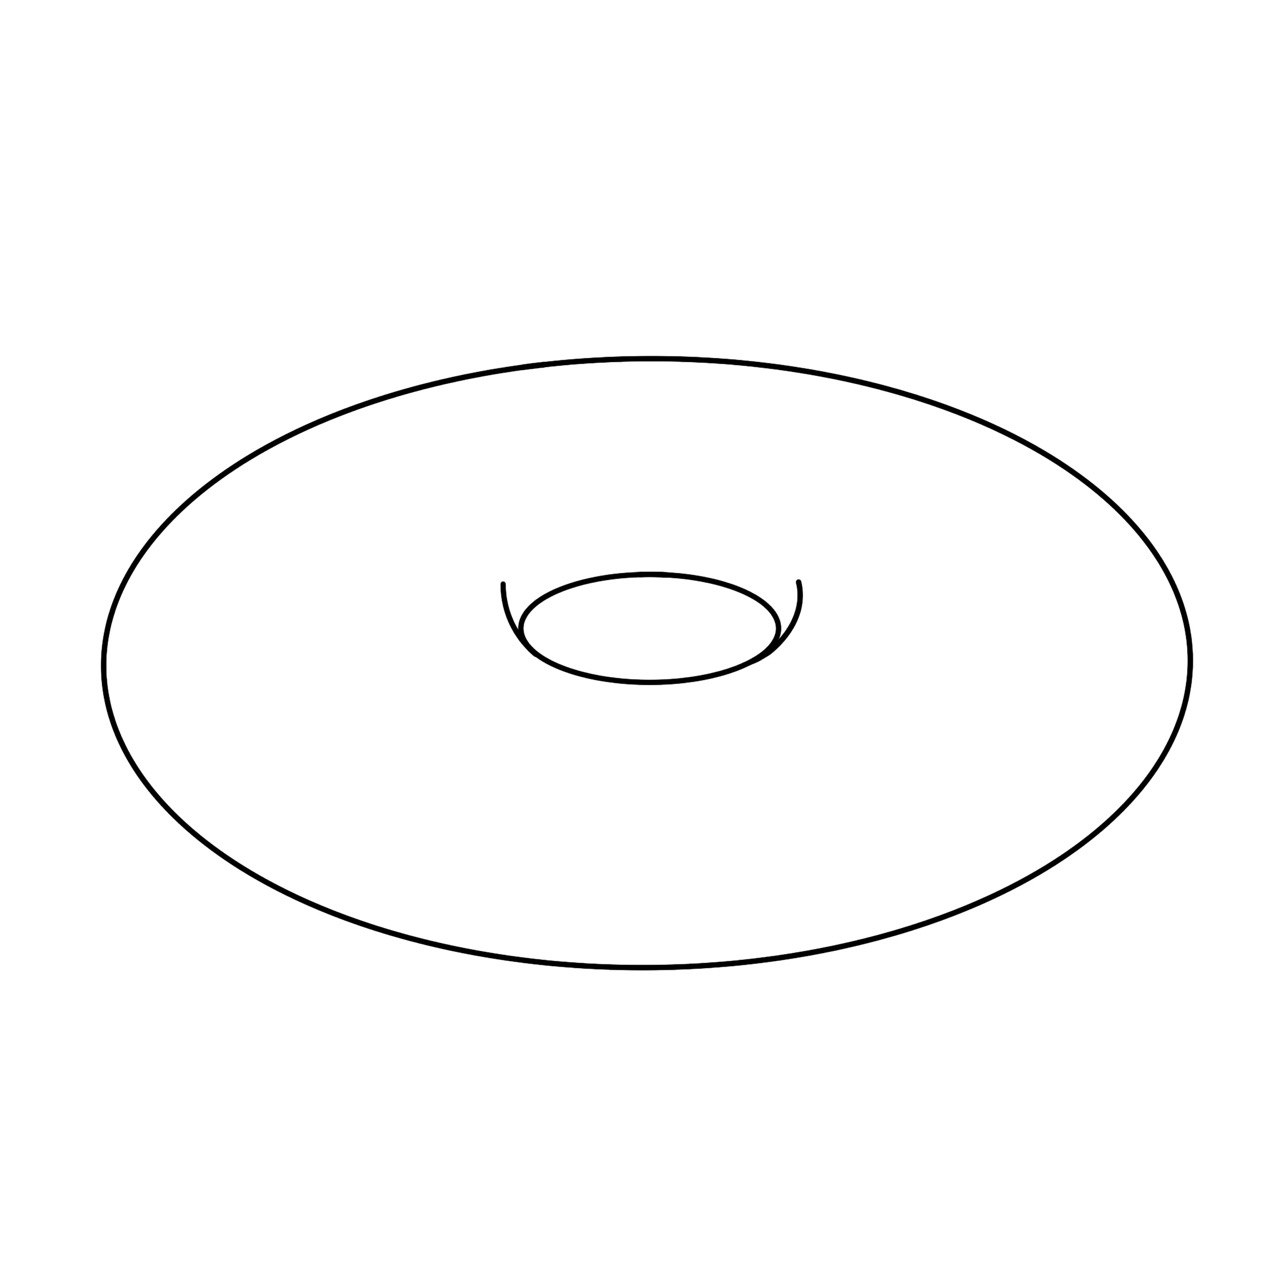
\includegraphics[width=\textwidth]{images/plain torus.jpg}
    \caption{Full-scale image of Figure~\ref{fig:torus}}
\end{figure}

\begin{figure}[H]
    \centering
    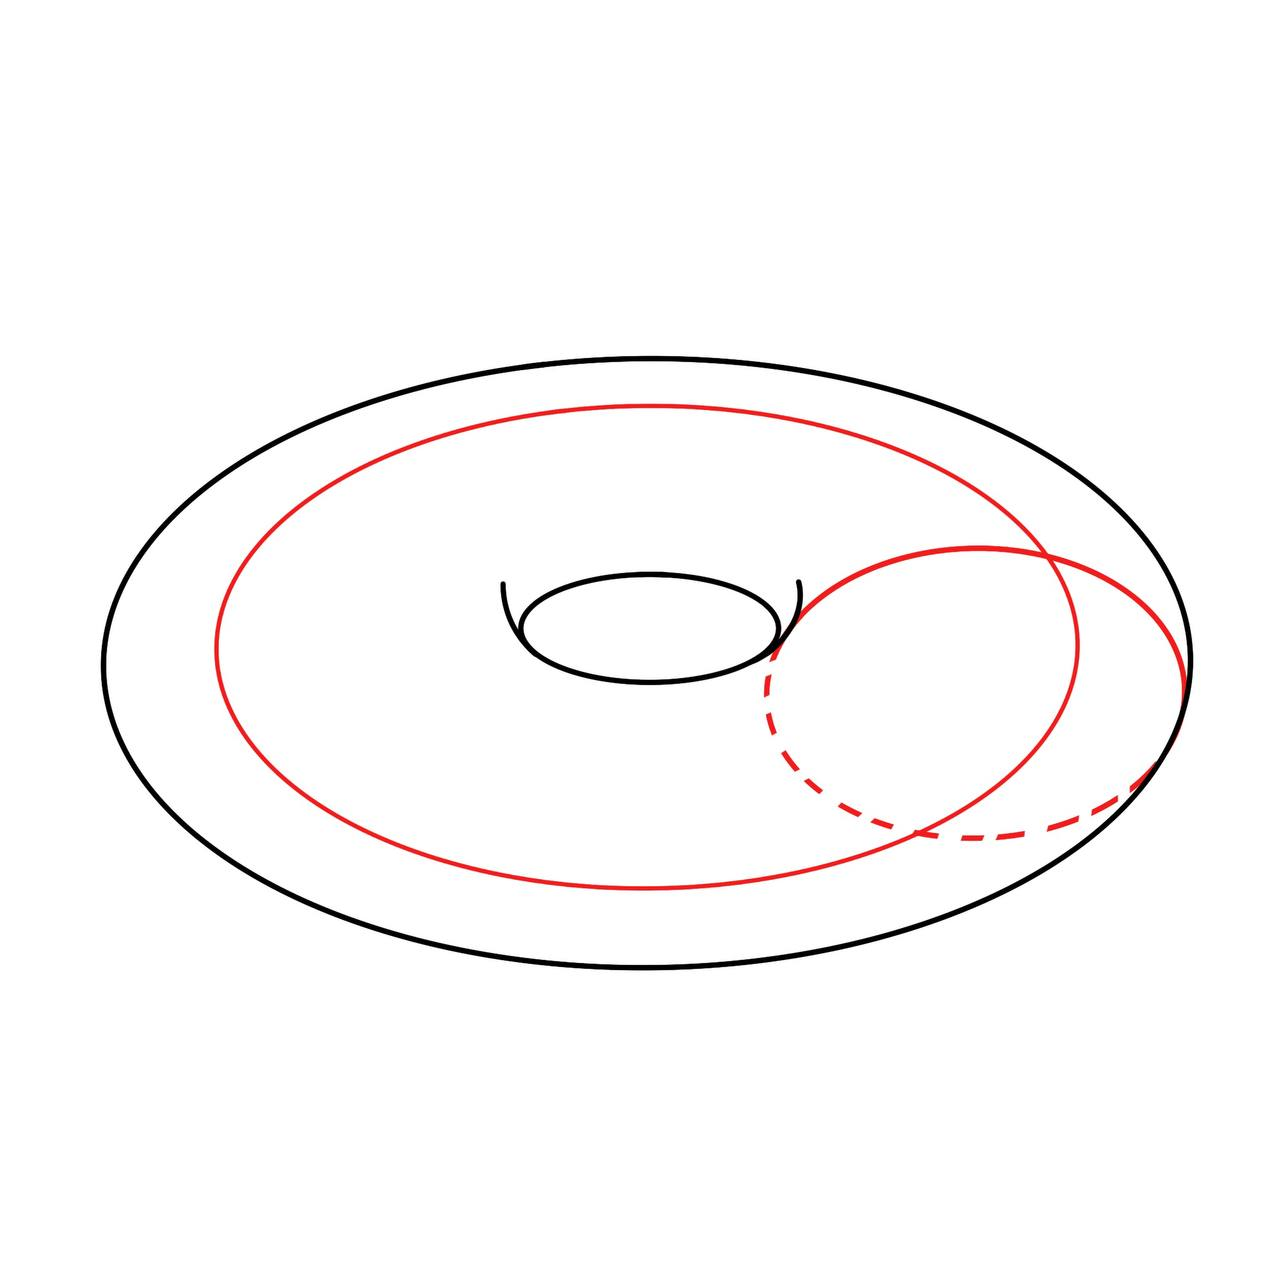
\includegraphics[width=\textwidth]{images/torus with curves.jpg}
    \caption{Full-scale image of Figure~\ref{fig:two circles}}
\end{figure}

\begin{figure}[H]
    \centering
    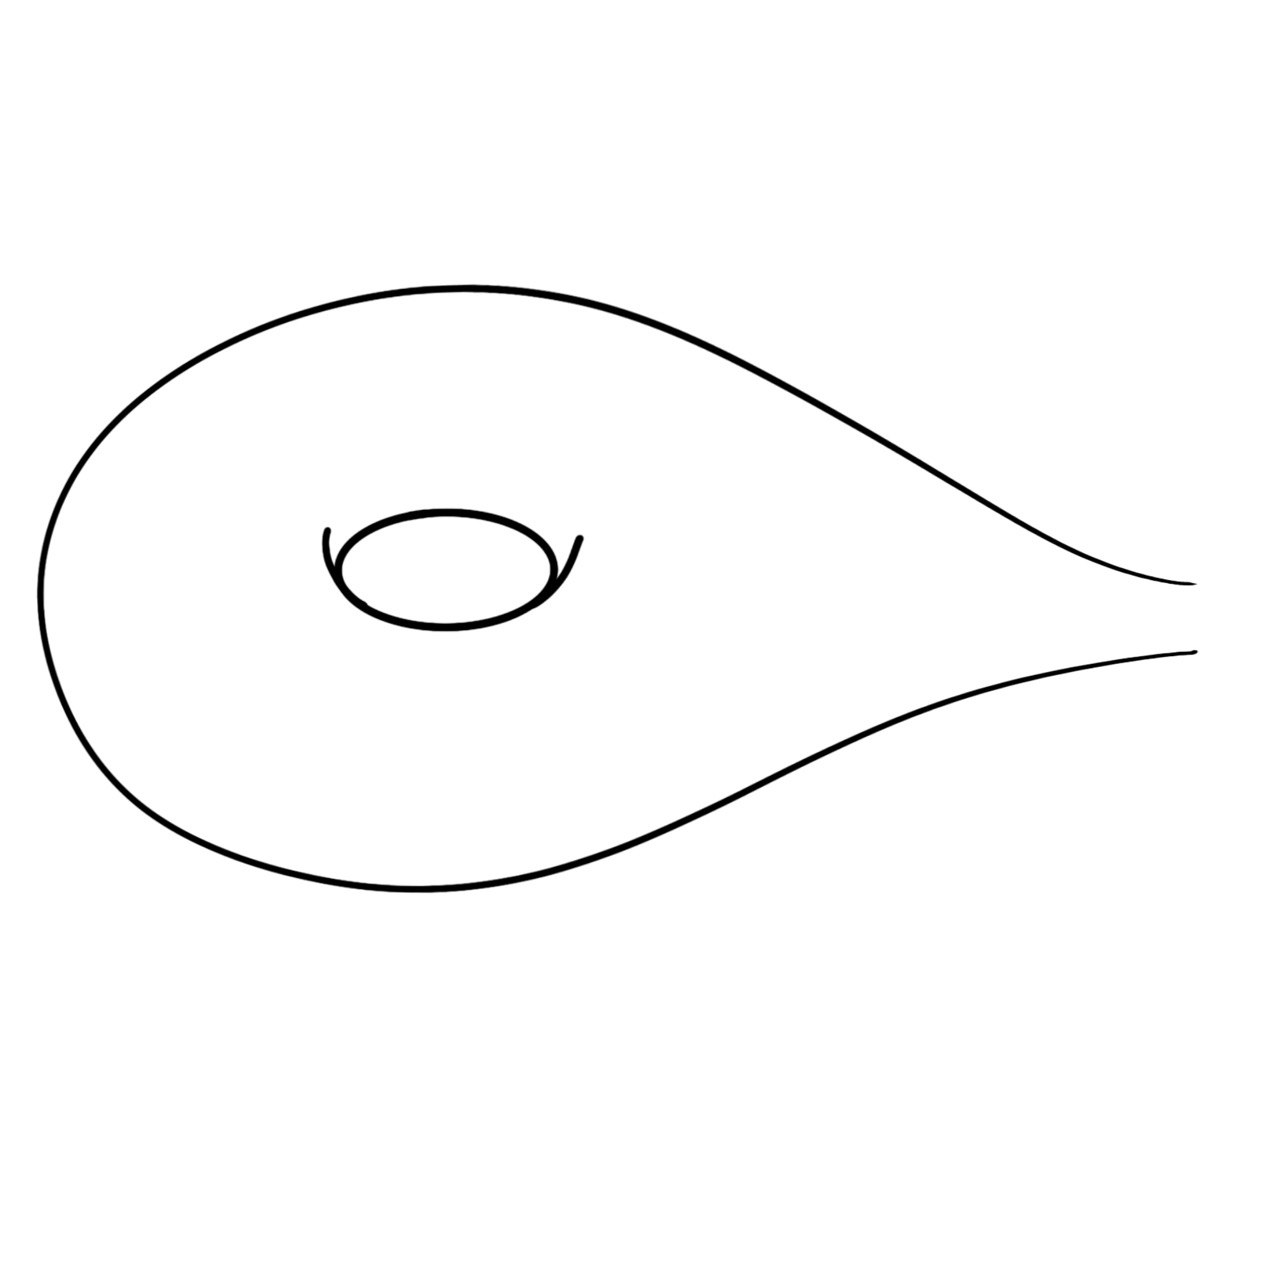
\includegraphics[width=\textwidth]{images/punctured torus.jpg}
    \caption{Full-scale image of Figure~\ref{fig:once punctured}}
\end{figure}

\begin{figure}[H]
    \centering
    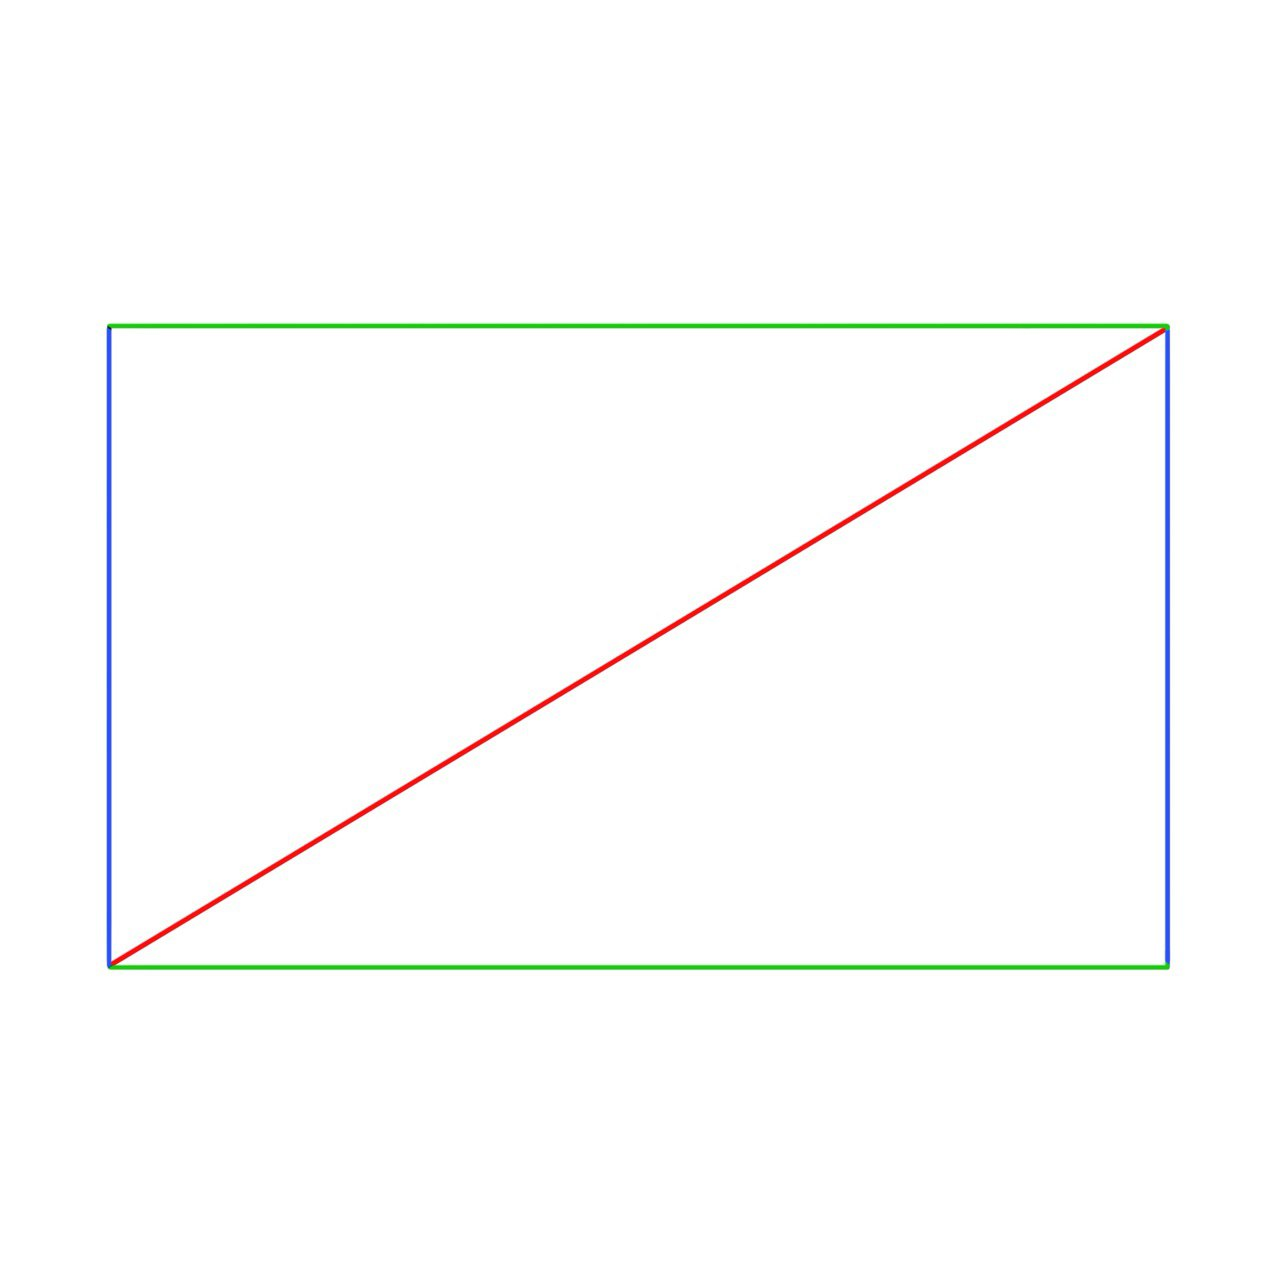
\includegraphics[width=\textwidth]{images/Universal Covering.jpg}
    \caption{Full-scale image of Figure~\ref{fig:covering}}
\end{figure}

\begin{figure}[H]
    \centering
    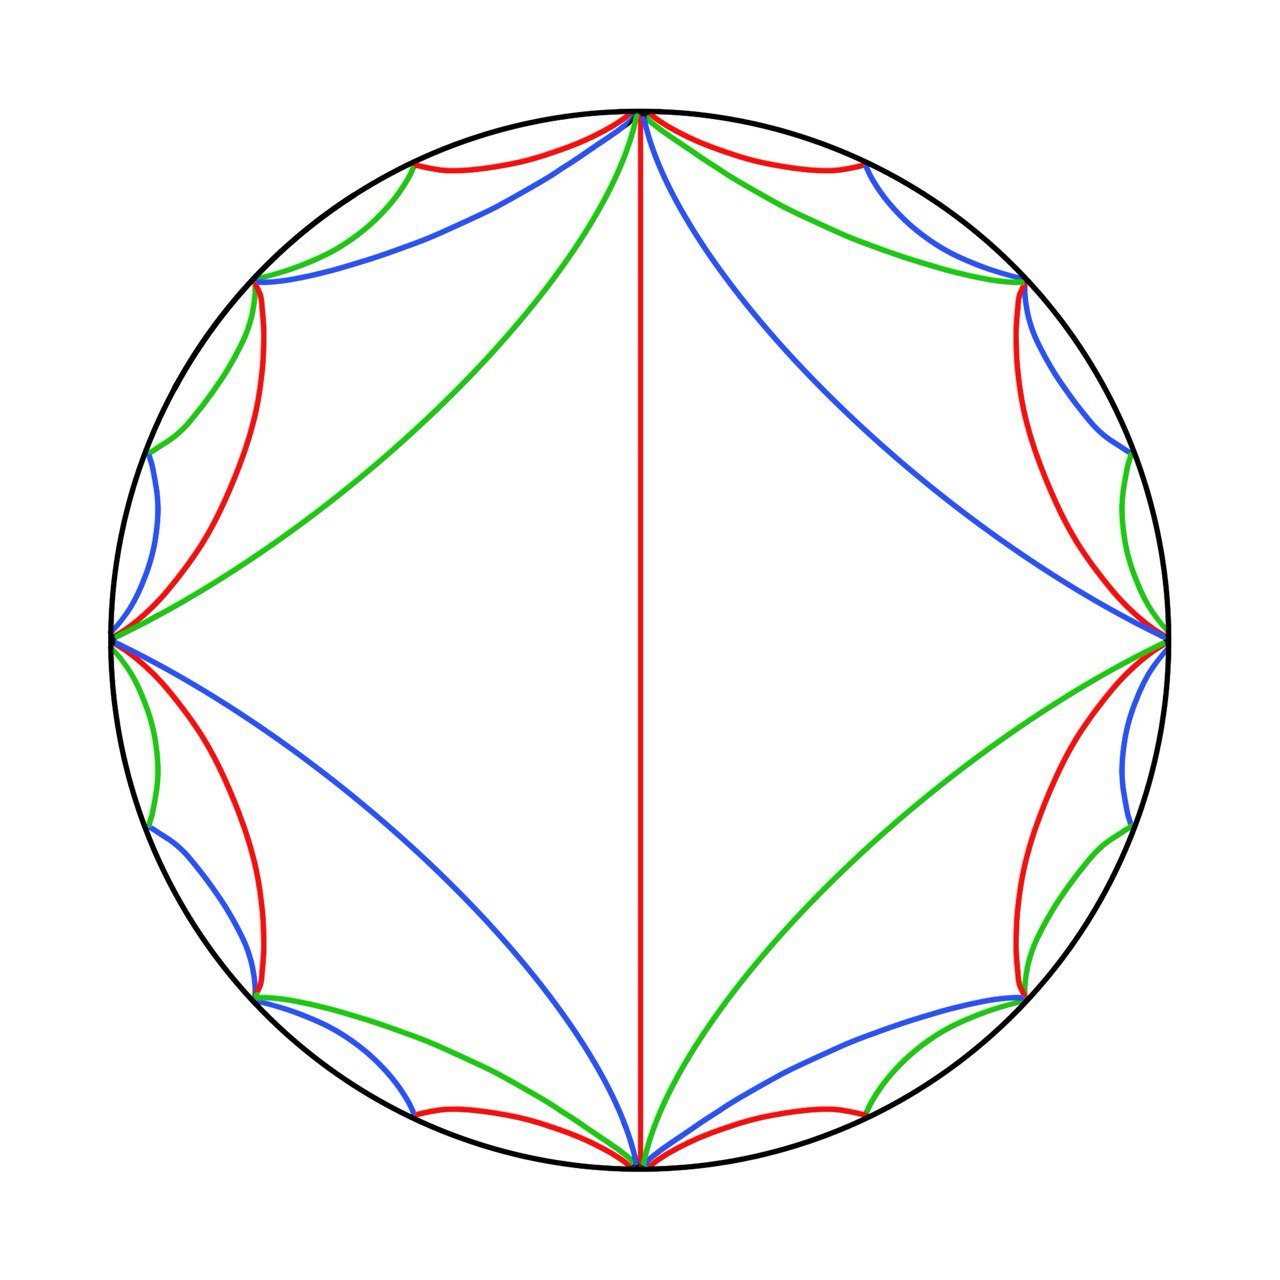
\includegraphics[width=\textwidth]{images/RS colored detailed.jpg}
    \caption{Full-scale image of Figure~\ref{fig:tesselated}}
\end{figure}

\begin{figure}[H]
    \centering
    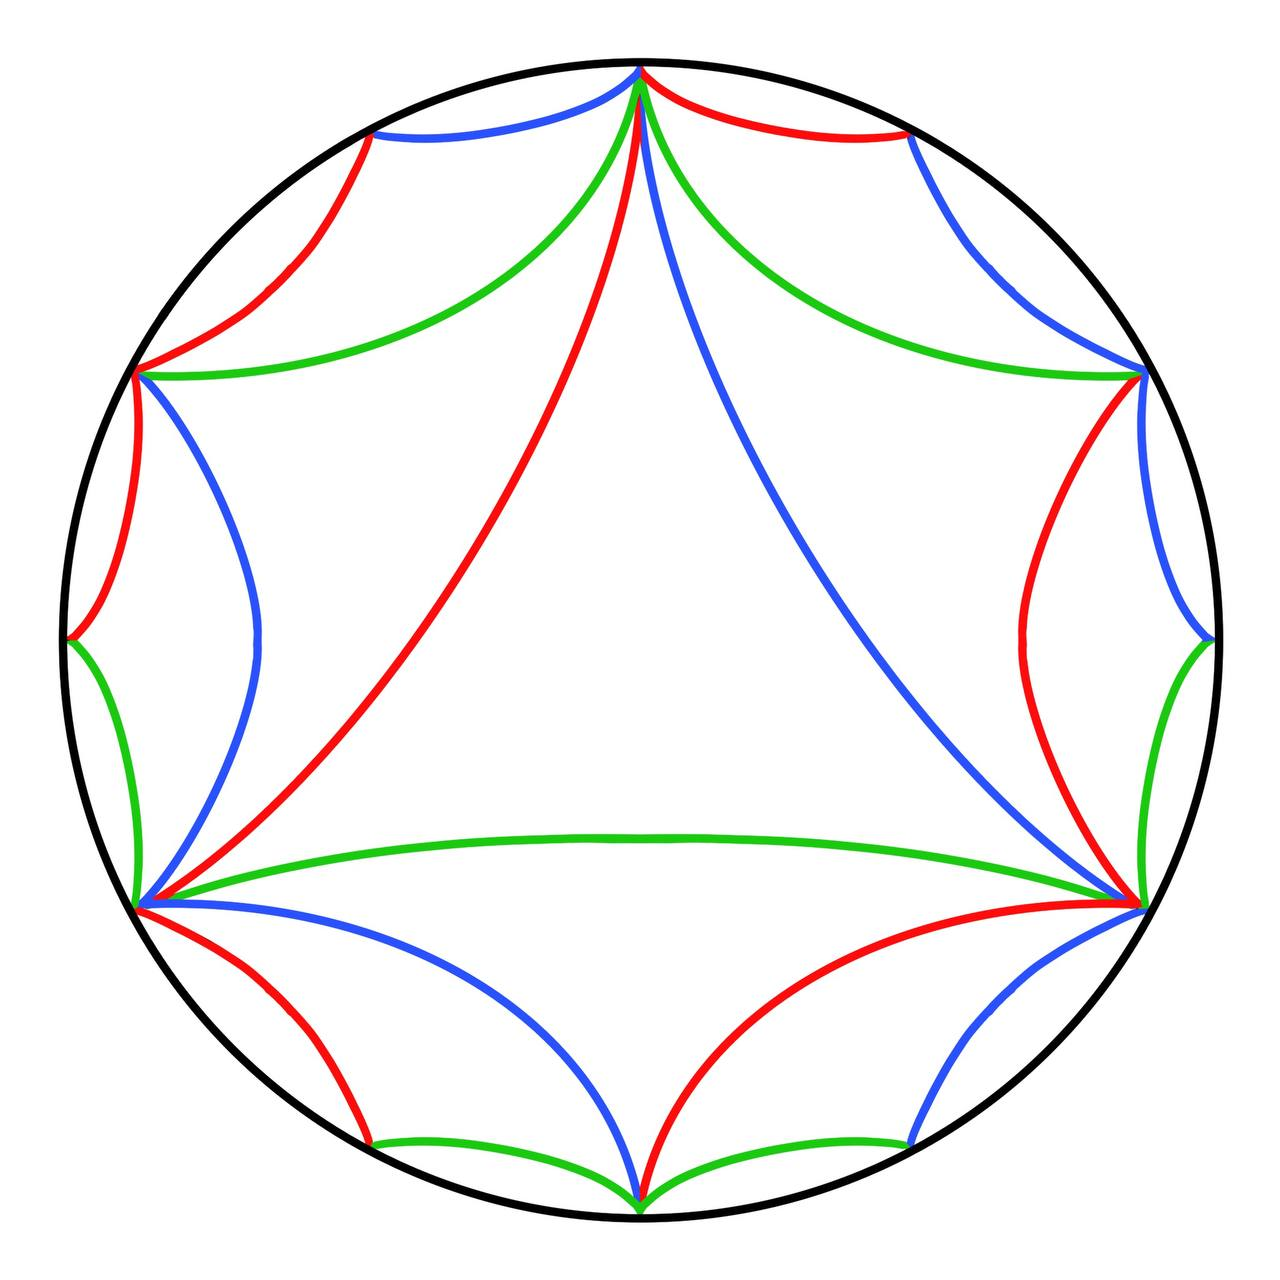
\includegraphics[width=\textwidth]{images/RS colored detailed 2.jpg}
    \caption{Full-scale image of Figure~\ref{fig:universal-covering-2}}
\end{figure}

\begin{figure}[H]
    \centering
    \includegraphics[width=\textwidth]{nn/a-100 b100 h40 d0.025}
    \caption{Full-scale image of Figure~\ref{fig:divergent cross-ratio}}
\end{figure}

\begin{figure}[H]
    \centering
    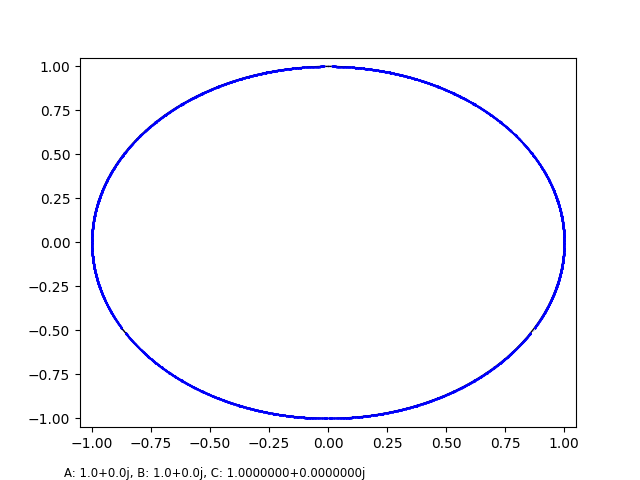
\includegraphics[width=\textwidth]{images/nn/a0 b0 h100 d0.001 auto xy.png}
    \caption{Full-scale image of Figure~\ref{fig:circle}}
\end{figure}

\begin{figure}[H]
    \centering
    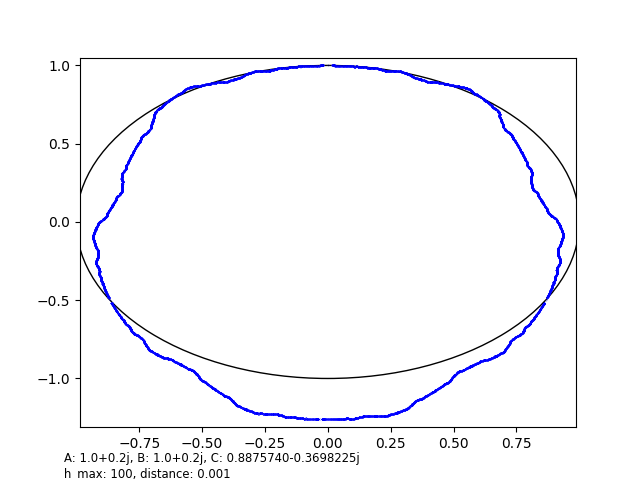
\includegraphics[width=\textwidth]{images/m/a.2,b.2,h100,d.0010.png}
    \caption{Full-scale image of Figure~\ref{fig:warped}}
\end{figure}

\begin{figure}[H]
    \centering
    \includegraphics[width=\textwidth]{images/m/a1,b1,h100,d.005.png}
    \caption{Full-scale image of Figure~\ref{fig:fractal}}
\end{figure}

\begin{figure}[H]
    \centering
    \includegraphics[width=\textwidth]{images/a2b2/a2,b2,h10,d0.png}
    \caption{Full-scale image of Figure~\ref{fig:a2b2h10}}
\end{figure}

\begin{figure}[H]
    \centering
    \includegraphics[width=\textwidth]{images/a2b2/a2,b2,h11,d0.png}
    \caption{Full-scale image of Figure~\ref{fig:a2b2h11}}
\end{figure}

\begin{figure}[H]
    \centering
    \includegraphics[width=\textwidth]{images/a2b2/a2,b2,h12,d0.png}
    \caption{Full-scale image of Figure~\ref{fig:a2b2h12}}
\end{figure}

\begin{figure}[H]
    \centering
    \includegraphics[width=\textwidth]{images/a2b2/a2,b2,h13,d0.png}
    \caption{Full-scale image of Figure~\ref{fig:a2b2h13}}
\end{figure}

\begin{figure}[H]
    \centering
    \includegraphics[width=\textwidth]{images/a2b2/a2,b2,h14,d0.png}
    \caption{Full-scale image of Figure~\ref{fig:a2b2h14}}
\end{figure}

\begin{figure}[H]
    \centering
    \includegraphics[width=\textwidth]{images/m/a3,b3,h100,d.005.png}
    \caption{Full-scale image of Figure~\ref{fig:m3}}
\end{figure}

\begin{figure}[H]
    \centering
    \includegraphics[width=\textwidth]{images/m/a5,b5,h100,d.005.png}
    \caption{Full-scale image of Figure~\ref{fig:m5}}
\end{figure}

\begin{figure}[H]
    \centering
    \includegraphics[width=\textwidth]{images/m/a10,b10,h100,d.005.png}
    \caption{Full-scale image of Figure~\ref{fig:m10}}
\end{figure}

\begin{figure}[H]
    \centering
    \includegraphics[width=\textwidth]{images/m/a100,b100,h100,d.0010.png}
    \caption{Full-scale image of Figure~\ref{fig:m100}}
\end{figure}

\begin{figure}[H]
    \centering
    \includegraphics[width=\textwidth]{images/m/a1000,b1000,h100,d.0005.png}
    \caption{Full-scale image of Figure~\ref{fig:m1,000}}
\end{figure}

\begin{figure}[H]
    \centering
    \includegraphics[width=\textwidth]{images/m/a10,000,b10,000,h100,d.0005.png}
    \caption{Full-scale image of Figure~\ref{fig:m10,000}}
\end{figure}

\begin{figure}[H]
    \centering
    \includegraphics[width=\textwidth]{images/m/a100,000,b100,000,h100,d.00075.png}
    \caption{Full-scale image of Figure~\ref{fig:m100,000}}
\end{figure}

\begin{figure}[H]
    \centering
    \includegraphics[width=\textwidth]{images/m/a150,000,b150,000,h100,d.0010.png}
    \caption{Full-scale image of Figure~\ref{fig:m150,000}}
\end{figure}

\begin{figure}[H]
    \centering
    \includegraphics[width=\textwidth]{images/m/a200,000,b200,000,h100,d.0010.png}
    \caption{Full-scale image of Figure~\ref{fig:m200,000}}
\end{figure}

\begin{figure}[H]
    \centering
    \includegraphics[width=\textwidth]{images/m/a1,000,000,b1,000,000,h100,d.005.png}
    \caption{Full-scale image of Figure~\ref{fig:m1,000,000}}
\end{figure}

\begin{figure}[H]
     \centering
     \includegraphics[width=\textwidth]{images/a1,b100,h100,d.01 custom xy.png}      
     \caption{Full-scale image of Figure~\ref{fig:a1b100}}
\end{figure}

\begin{figure}[H]
        \includegraphics[width=\textwidth]{images/a100,b1,h100,d.05.png}
         \caption{Full-scale image of Figure~\ref{fig:a100b1}}
\end{figure}

\begin{figure}[H]
    \centering
    \includegraphics[width=\textwidth]{images/a1,b100,h100,d.01 custom xy.png}         \includegraphics[width=\textwidth]{images/a1,b100,h100,d.05.png}
    \caption{Full-scale image of Figure~\ref{fig:a1b100range}}
\end{figure}

\begin{figure}[H]
    \centering
    \includegraphics[width=\textwidth]{images/a2b2/a2,b2,h14,d0 custom bounds.png}
    \includegraphics[width=\textwidth]{images/a2b2/a2,b2,h14,d0.png}
    \caption{Full-scale image of Figure~\ref{fig:a2b2h14range}}
\end{figure}

\begin{figure}[H]
    \centering
    \includegraphics[width=\textwidth]{images/nn/a0 b0 h100 d0.001 fixed xy.png}
    \caption{Full-scale image of Figure~\ref{fig:n0}}
\end{figure}

\begin{figure}[H]
    \centering
    \includegraphics[width=\textwidth]{images/nn/a-1 b1 h30 d0.01.png}
    \caption{Full-scale image of Figure~\ref{fig:n1}}
\end{figure}

\begin{figure}[H]
    \centering
    \includegraphics[width=\textwidth]{images/nn/a-2 b2 h30 d0.01.png}
    \caption{Full-scale image of Figure~\ref{fig:n2}}
\end{figure}

\begin{figure}[H]
    \centering
    \includegraphics[width=\textwidth]{images/nn/a-2.5 b2.5 h30 d0.01.png}
    \caption{Full-scale image of Figure~\ref{fig:n2.5}}
\end{figure}

\begin{figure}[H]
    \centering
    \includegraphics[width=\textwidth]{images/nn/a-3 b3 h40 d0.025.png}
    \caption{Full-scale image of Figure~\ref{fig:n3}}
\end{figure}

\begin{figure}[H]
    \centering
    \includegraphics[width=\textwidth]{images/nn/a-3.5 b3.5 h30 d0.01.png}
    \caption{Full-scale image of Figure~\ref{fig:n3.5}}
\end{figure}

\begin{figure}[H]
    \centering
    \includegraphics[width=\textwidth]{images/nn/a-4 b4 h30 d0.01.png}
    \caption{Full-scale image of Figure~\ref{fig:n4}}
\end{figure}

\begin{figure}[H]
    \centering
    \includegraphics[width=\textwidth]{images/nn/a-5 b5 h30 d0.01.png}
    \caption{Full-scale image of Figure~\ref{fig:n5}}
\end{figure}

\begin{figure}[H]
    \centering
    \includegraphics[width=\textwidth]{images/nn/a-10 b10 h30 d0.01.png}
    \caption{Full-scale image of Figure~\ref{fig:n10}}
\end{figure}

\begin{figure}[H]
    \centering
    \includegraphics[width=\textwidth]{images/nn/a-100 b100 h40 d0.025.png}
    \caption{Full-scale image of Figure~\ref{fig:n100}}
\end{figure}


\end{document}
